
%%%%%%%%%%%%%%%%%%%%%%%%%%%%%%%%%%%%%%%%%%%%%%%%%%%%%%%%%%
    \documentclass[twoside,11pt]{article}
    %%%%% PACKAGES %%%%%%
    \usepackage{ctex}
    \usepackage{pgm2016}
    \usepackage{amsmath}
    \usepackage{algorithm}
    \usepackage[noend]{algpseudocode}
    \usepackage{subcaption}
    \usepackage[english]{babel}	
    \usepackage{paralist}	
    \usepackage[lowtilde]{url}
    \usepackage{fixltx2e}
    \usepackage{listings}
    \usepackage{color}
    \usepackage{enumerate}
    \usepackage{booktabs}
    \usepackage{multicol}
    \usepackage{auto-pst-pdf}
    \usepackage{pst-all}
    \usepackage{pstricks-add}
	\usepackage{comment}
	\usepackage{fancybox}
    \usepackage[hidelinks]{hyperref}
    \usepackage{bbding}

    %%%%% MACROS %%%%%%
    \algrenewcommand\Return{\State \algorithmicreturn{} }
    \algnewcommand{\LineComment}[1]{\State \(\triangleright\) #1}
    \renewcommand{\thesubfigure}{\roman{subfigure}}
    \definecolor{codegreen}{rgb}{0,0.6,0}
    \definecolor{codegray}{rgb}{0.5,0.5,0.5}
    \definecolor{codepurple}{rgb}{0.58,0,0.82}
    \definecolor{backcolour}{rgb}{0.95,0.95,0.92}
    \lstdefinestyle{mystyle}{
       backgroundcolor=\color{backcolour},  
       commentstyle=\color{codegreen},
       keywordstyle=\color{magenta},
       numberstyle=\tiny\color{codegray},
       stringstyle=\color{codepurple},
       basicstyle=\footnotesize,
       breakatwhitespace=false,        
       breaklines=true,                
       captionpos=b,                    
       keepspaces=true,                
       numbers=left,                    
       numbersep=5pt,                  
       showspaces=false,                
       showstringspaces=false,
       showtabs=false,                  
       tabsize=2
    }
    \lstset{style=mystyle}
%%%%%%%%%%%%%%%%%%%%%%%%%%%%%%%%%%%%%%%%%%%%%%%%%%%%%%%%%% 

%%%%%%%%%%%%%%%%%%%%%%%%%%%%%%%%%%%%%%%%%%%%%%%%%%%%%%%%%% 
\newcommand\courseName{Programming in Python}
\newcommand\semester{Fall 2022}
\newcommand\assignmentNumber{1}
\newcommand\studentName{\Large \centering 任课教师: 张涵翠\\王旭刚 2020329621074\\韦杨婧 2020329621199\\池胤杰 2020329621049\\计算机科学与技术全英文授课班20(1)\\}
\newcommand\studentEmail{Email:castamerego@gmail.com}
\newcommand\studentNumber{2020329621074, 2020329621199, 2020329621049}
\newcommand\projectname{Read-Book "智能知识侦查助手"}
\newcommand\studentClass{\centering}
%%%%%%%%%%%%%%%%%%%%%%%%%%%%%%%%%%%%%%%%%%%%%%%%%%%%%%%%%%
\renewcommand{\thefootnote}{\fnsymbol{footnote}}
\newenvironment{boxedlaw}[1]
{\begin{Sbox}\begin{minipage}{#1}\setcounter{mpfootnote}{\value{footnote}}}
		{\end{minipage}\end{Sbox}\begin{center}\shadowbox{\TheSbox}
		\setcounter{footnote}{\value{mpfootnote}}\end{center}}

\renewcommand*\thempfootnote{\fnsymbol{mpfootnote}}



\ShortHeadings{Coursework of ZSTU - \courseName}{\projectname}
    
\begin{document}

\begin{figure}[H]
    \centering
    
\includegraphics[width=1\columnwidth]{figures/zstu-logo.png}
\end{figure}

\title{\Huge Python 程序设计\\ \vspace{1.5cm} Read-Book ``智能知识侦查助手"(9) \\ \vspace{1.5cm} \huge 2022-2023-1 \\ \vspace{0.8cm}}

\author{\name \studentName{}
    \addr
}

\maketitle
\thispagestyle{empty}
\newpage



\phantomsection\addcontentsline{toc}{section}{Author}\tolerance=500

\begin{center}
    王旭刚\textsuperscript{1*},
    韦杨婧\textsuperscript{2},
    池胤杰\textsuperscript{3}
    \\
    \bigskip
    \textbf{1} Leader, back-end design and implementation
    \\
    \textbf{2} Team member, front-end design and implementation
    \\
    \textbf{3} Team member, question data collect
    \\
    \bigskip
    %
\end{center}



\phantomsection\addcontentsline{toc}{section}{Abstruct}\tolerance=500

\begin{center}
    \Large\textbf{Abstruct}
\end{center}

In this Safehome Project Design, there are four parts : 1. Determine actors and the corresponding functions 2. For each function write story to extract actions 3. Write formal (Structured) use-cases 4. Create swimlane diagram for each use-case.

\pagenumbering{Roman}
\newpage



\phantomsection\addcontentsline{toc}{section}{课题执行(文档修订)记录表}\tolerance=500

\begin{center}
    \Large \textbf{课题执行(文档修订)记录表}
\end{center}

\begin{table}[H]
    \centering
    \caption{课题执行(文档修订)记录表}
    \setlength{\tabcolsep}{9mm}{
        \begin{tabular}{|c|c|c|c|c|}
            \hline
            日期       & 版本 & 修订内容 & 执行人 & 修订人 \\
            \hline
            2022.11.06 & 1.0  & 分析需求 & 王旭刚 & 韦杨婧 \\
            \hline
        \end{tabular}}

    \label{tab:tab1}
\end{table}

\newpage



\begin{center}
    \tableofcontents
\end{center}
\thispagestyle{empty}
\newpage



\pagenumbering{arabic}


\section{系统设计}
\subsection{概要设计}
\subsubsection{系统框架设计}
\subsubsection{系统功能设计}
\subsection{功能设计}
\subsubsection{功能1}
\subsubsection{功能2}
\subsection{数据库设计}

\begin{table}[H]
    \centering
    \caption{书籍储数据存---数据库设计}
    \begin{tabular}{|l|l|c|c|c|}
        \hline
        Attribute     & Translation & Type    & Chinese Book & Foreign Book \\
        \hline
        Id            & 排名        & int     & \Checkmark   & \Checkmark   \\
        \hline
        Name          & 书名        & varchar & \Checkmark   & \Checkmark   \\
        \hline
        Author        & 作者        & varchar & \Checkmark   & \Checkmark   \\
        \hline
        Country       & 国家        & varchar & \Checkmark   & \Checkmark   \\
        \hline
        Publisher     & 出版社      & varchar & \Checkmark   & \Checkmark   \\
        \hline
        Year          & 出版日期    & varchar & \Checkmark   & \Checkmark   \\
        \hline
        Page          & 页数        & varchar & \Checkmark   & \Checkmark   \\
        \hline
        Price         & 定价        & varchar & \Checkmark   & \Checkmark   \\
        \hline
        Frame         & 装帧        & varchar & \Checkmark   & \Checkmark   \\
        \hline
        Category      & 丛书        & varchar & \Checkmark   & \Checkmark   \\
        \hline
        Isbn          & isbn码      & varchar & \Checkmark   & \Checkmark   \\
        \hline
        Star          & 评分        & float   & \Checkmark   & \Checkmark   \\
        \hline
        Comment num   & 评价数量    & int     & \Checkmark   & \Checkmark   \\
        \hline
        Brief         & 简介        & varchar & \Checkmark   & \Checkmark   \\
        \hline
        Douban bookid & 豆瓣id      & varchar & \Checkmark   & \Checkmark   \\
        \hline
        Link          & 链接        & varchar & \Checkmark   & \Checkmark   \\
        \hline
        Name o        & 原作名      & varchar & \XSolid      & \Checkmark   \\
        \hline
        Trans         & 译者        & varchar & \XSolid      & \Checkmark   \\
        \hline
    \end{tabular}

    \label{tab:tabforbook}
\end{table}

\begin{table}[H]
    \centering
    \caption{用户数据储存---数据库设计}
    \setlength{\tabcolsep}{11mm}{
        \begin{tabular}{|c|c|c|}
            \hline
            Attribute & Type    & Translation \\

            \hline
            Id        & int     & 编号        \\
            \hline
            Name      & varchar & 姓名        \\
            \hline
            Gender    & char    & 性别        \\
            \hline
            Telephone & varchar & 电话        \\
            \hline
            Password  & varchar & 密码        \\
            \hline
            Brief     & varchar & 简介        \\
            \hline
        \end{tabular}
    }
    \label{tab:tabforuser}
\end{table}


\begin{table}[H]
    \centering
    \caption{问题储存---数据库设计}
    \setlength{\tabcolsep}{7mm}{
        \begin{tabular}{|c|c|c|c|}
            \hline
            Attribute    & Type    & Translation    & Note                       \\
            \hline
            Id           & int     & 关联书本的id   &                            \\
            \hline
            Question     & varchar & 问题           &                            \\
            \hline
            Type         & int     & 类别           & 0-判断, 1-单选, 2-多选     \\
            \hline
            Question num & int     & 选项数量       &                            \\
            \hline
            C1           & varchar & 选项1          &                            \\
            \hline
            C2           & varchar & 选项2          &                            \\
            \hline
            C3           & varchar & 选项3          &                            \\
            \hline
            C4           & varchar & 选项4          &                            \\
            \hline
            Ans          & varchar & 正确选项       & 必须与某个选项完全相同     \\
            \hline
            Category     & varchar & 问题内容的类别 & 如: 问作者, 书中人物, 情节 \\
            \hline
        \end{tabular}
    }
    \label{tab:tabforquestion}
\end{table}

\section{系统实现}
\subsection{前端实现}
\subsection{后端实现}



\section{结束语}
\subsection{总结}
\subsection{不足与展望}




In this project design, we need to design a \emph{SafeHome System} appling the \textbf{Scenario-Based Modeling}. Using which if you want to understand how users want to interact with a system\cite{roger2015software}. In all, the whole project can be devided into four parts:
\begin{enumerate}
    \item Determine actors and the corresponding functions
    \item For each function write story to extract actions
    \item Write formal (Structured) use-cases
    \item Create swimlane diagram for each use-case
\end{enumerate}

\section{Actors and Functions}

\subsection{Actors}

Actors are those individuals or systems that will interact with the application\cite{Lance2018Creating}. When defining the actors, one may just think of the perspective from the \emph{C-S} structure, that is, client(Homeowner) and server(Administrator). But there are several other actors that interact with the system from not just a software perspective, but also from an external software and hardware perspective. In addition, these actors should be broken down into two categories, primary and secondary. The primary actor is the actor that is directly interacting with the system to achieve a goal. The secondary actor is the actor is external to the system, but is called upon to help complete a goal. So here are my design for Safehome actors:
\begin{itemize}
    \item Primary Actor:
          \begin{itemize}
              \item Administrator
              \item Homeowner
          \end{itemize}

    \item Secondary Actor:
          \begin{itemize}
              \item Camera
              \item Sensor
          \end{itemize}
\end{itemize}

\subsection{Functions}
After we determined the Actors, we need to consider what functions does these actors need to perform. And from those actions, we can derive Use-Cases. So here are my design for Safehome functions:
\begin{itemize}
    \item Administrator:
          \begin{enumerate}
              \item Register new Homeowner
              \item Delete Homeowner
              \item Add/Remove Camera
              \item Add/Remove Sensor
              \item Contact Homeowner/Emergency service when Emergency
          \end{enumerate}
    \item Homeowner:
          \begin{itemize}
              \item Information Security Related:
                    \begin{enumerate}
                        \setcounter{enumi}{5}
                        \item Login (Validate user ID and password)
                        \item Logout
                        \item Modify profile
                    \end{enumerate}
              \item House Safety Related:
                    \begin{enumerate}
                        \setcounter{enumi}{8}
                        \item View Cameras
                        \item Zoom selected Camera
                        \item Show thumbnails of all Cameras
                        \item Record and Replay Camera video
                        \item Activate/Deactivate Cameras
                        \item Activate/Deactivate Sensors
                        \item View history records
                    \end{enumerate}
          \end{itemize}

    \item Camera:
          \begin{enumerate}
              \setcounter{enumi}{15}
              \item Activate/Deactivate
              \item Zoom in/out
              \item Record Video
          \end{enumerate}
    \item Sensor:
          \begin{enumerate}
              \setcounter{enumi}{18}
              \item Activate/Deactivate
              \item Gather data
              \item Send data to Homeowner/Administrator
          \end{enumerate}
\end{itemize}
\newpage

\section{User Scenario}

The scenario approach is a high level description with the key components listed out in a stepwise manner\cite{Lance2018Creating}. To better illustrate the Use-Cases of the actors, we need to come up with a narrative scenario for each Use-Case, a lateral description, without side interactions. After that, all we need to do is conduct a step-by-step analysis of the scenario to extract the actions.


% Login to the system
\subsection{Scenario 1: Login to the system}

\textbf{Actor:}Homeowner

\textbf{Scenario story:}

If I want to check the status of my house, I need to login to the system. I may choose to login using my PC or my mobile phone with the application or a browser to the \emph{SafeHome Products} website. After I input my user ID and password, the system will validate my user ID and password. If the user ID and password are correct, I will be able to login to the system. If the user ID and password are incorrect, I will be prompted to re-enter my user ID and password. And once I login to the system, I will be able to view the status of my house and will have access to all functionality my installed \emph{SafeHome} system.

\textbf{Actions:}

\begin{enumerate}
    \item The homeowner logs onto the \emph{SafeHome Products} website on his PC or opens the \emph{SafeHome} application on his mobile phone.
    \item The homeowner inputs his user ID and password.
    \item The system displays all major functionalities of the \emph{SafeHome} system.
\end{enumerate}

% Modify profile

\subsection{Scenario 2: Modify Profile}

\textbf{Actor:}Homeowner

\textbf{Scenario story:}

If I want to change my user ID, password, or personal information, I may need to modify the profile. I may choose to modify my profile using my PC or my mobile phone with the application or a browser to the \emph{SafeHome Products} website. After I login to the system, I will be able click on my avatar to check my profile. And in that new page, I can click on the "Modify Profile" to change my user ID, password, or personal information. And once I modify my profile, I will be able to login to the system with the new user ID and password.

\textbf{Actions:}

\begin{enumerate}
    \item The homeowner logs onto the \emph{SafeHome Products} website on his PC or opens the \emph{SafeHome} application on his mobile phone.
    \item The homeowner inputs his user ID and password.
    \item The system displays all major functionalities of the \emph{SafeHome} system.
    \item The homeowner clicks on his avatar to check his profile.
    \item The system displays the profile page.
    \item The homeowner clicks on the "Modify Profile" button.
    \item The system displays the modify profile page.
    \item The homeowner click on the field he wants to modify and input.
    \item The homeowner click on the "Save" button.
\end{enumerate}

% View Cameras

\subsection{Scenario 3: Access Camera Surveillance}

\textbf{Actor:}Homeowner

\textbf{Scenario story:}

If I'm at a remote location and want to check the status of my house, I may need to access the camera Surveillance. I can use my PC or my mobile phone with the application or a browser to the \emph{SafeHome Products} website. After I successfully logged in, I will be able to view the status of my house and will have access to all functionality my installed \emph{SafeHome} system. And in the \emph{SafeHome} system, I can click on the "Surveillance" button to look at the thumbnail snapshots from all cameras simultaneously by default. And I can click on any camera window to watch the live video from that camera. And I can also click on the "zoom in" or "zoom out" button to zoom in or zoom out the camera. If I want to switch to another camera, I can choose to press "go back" button to go back to previous window of thumbnail snapshots display or to click the left or right button to go through the cameras one by one.

\textbf{Actions:}

\begin{enumerate}
    \item The homeowner logs onto the \emph{SafeHome Products} website on his PC or opens the \emph{SafeHome} application on his mobile phone.
    \item The homeowner inputs his user ID and password.
    \item The system displays all major functionalities of the \emph{SafeHome} system.
    \item The homeowner clicks on the "Surveillance" button.
    \item The system displays the thumbnail snapshots from all cameras simultaneously by default.
    \item The homeowner clicks on any camera window to watch the live video from that camera.
    \item The homeowner clicks on the "zoom in" or "zoom out" button to zoom in or zoom out the camera.
    \item The homeowner clicks on the "go back" button to go back to previous window of thumbnail snapshots display. Or clicks on the left or right button to go through the cameras one by one.
\end{enumerate}

% Activate/Deactivate 

\subsection{Scenario 4: Activate and Deactivate the Cameras and Sensors}

\textbf{Actor:}Homeowner

\textbf{Secondary Actor:}Cameras, Sensors

\textbf{Scenario story:}

If I'm currently in home, I may need to deactivate Cameras and Sensors out of privacy or energy-saving purpose. And when I left home, I may need to activate the Cameras and Sensors for security purpose. I can use my PC or my mobile phone with the application or a browser to the \emph{SafeHome Products} website. After I successfully logged in, I can click the "Back Home" button to deactivate Cameras and Sensors, and click the "Leave Home" button to activate Cameras and Sensors.

\textbf{Actions:}

\begin{enumerate}
    \item The homeowner logs onto the \emph{SafeHome Products} website on his PC or opens the \emph{SafeHome} application on his mobile phone.
    \item The homeowner inputs his user ID and password.
    \item The system displays all major functionalities of the \emph{SafeHome} system.
    \item The homeowner clicks the "Back Home" button.
    \item The system deactivates Cameras and Sensors.
    \item The homeowner clicks the "Leave Home" button.
    \item The system activates Cameras and Sensors.
\end{enumerate}

% Add/Delete Homeowner

\subsection{Scenario 5: Register new Homeowner/Delete Homeowner}

\textbf{Actor:} Administrator

\textbf{Scenario story:}

If the Homeowner want to add new family member to the system, the Administrator can register new Homeowner. If the homeowner want to remove a family member from the system, the Administrator can delete the Homeowner. The Administrator can use his PC to open the \emph{SafeHome Products} Software. After he successfully logged in, he can click on the "Homeowner" button to check the list of all Homeowners. And he can click on the "Add Homeowner" button to add new Homeowner. He then need to input the new Homeowner's user ID, password, and personal information. And he can click on the "Delete Homeowner" button and select the Homeowner he want to delete to delete a Homeowner.

\textbf{Actions:}
\begin{enumerate}
    \item The Administrator opens the \emph{SafeHome Products} Software on his PC.
    \item The Administrator click on the "Homeowner" button.
    \item The system displays the list of all Homeowners.
    \item The Administrator click on the "Add Homeowner" button.
    \item The system displays the "Add Homeowner" page.
    \item The Administrator inputs the new Homeowner's user ID, password, and personal information.
    \item The Administrator click on the "Save" button.
    \item The system adds the new Homeowner to the system.
    \item The Administrator click on the "Delete Homeowner" button.
    \item The system displays the "Delete Homeowner" page.
    \item The Administrator selects the Homeowner he wants to delete.
    \item The Administrator click on the "Delete" button.
    \item The system deletes the selected Homeowner from the system.
\end{enumerate}

% Add/Delete Camera/Sensor

\subsection{Scenario 6: Add/Remove Camera or Sensor}

\textbf{Actor:}Administrator

\textbf{Secondary Actor:}Cameras, Sensors

\textbf{Scenario story:}

If the Homeowner bought a new Camera or Sensor, the Administrator can add the new Camera or Sensor to the system. If the current Camera or Sensor broken down, the Administrator can remove the Camera or Sensor from the system. The Administrator can use his PC to open the \emph{SafeHome Products} Software. After he successfully logged in, he can click on the "Camera" button to check the list of all Cameras. And he can click on the "Add Camera" button to add new Camera. He then need to input the new Camera's ID, location, and type. And he can click on the "Delete Camera" button and select the Camera he want to delete to delete a Camera. The same procedure applies to the Sensors.

\textbf{Actions:}
\begin{enumerate}
    \item The Administrator opens the \emph{SafeHome Products} Software on his PC.
    \item The Administrator click on the "Camera" button.
    \item The system displays the list of all Cameras(Camera contents are not included).
    \item The Administrator click on the "Add Camera" button.
    \item The system displays the "Add Camera" page.
    \item The Administrator inputs the new Camera's ID, location, and type.
    \item The Administrator click on the "Save" button.
    \item The system adds the new Camera to the system.
    \item The Administrator click on the "Delete Camera" button.
    \item The system displays the "Delete Camera" page.
    \item The Administrator selects the Camera he wants to delete.
    \item The Administrator click on the "Delete" button.
    \item The system deletes the selected Camera from the system.
    \item The same Actions applies to the Sensors.
\end{enumerate}


% Emergency

\subsection{Scenario 7: Contact Homeowneror Emergency service when Emergency occurs}

\textbf{Actor:}Administrator

\textbf{Secondary Actor:}Homeowner, Sensors, Cameras

\textbf{Scenario story:}

If the Sensor detected an Emergency or the Homeowner pressed the Emergency button, the Administrator will be notified. Then the Administrator will check the Surveillance video to determine if the Emergency is real. If the Emergency is real, the Administrator will contact the Homeowner and the Emergency service.

\textbf{Actions:}
\begin{enumerate}
    \item The Sensors detectedan Emergency or the Homeowner pressed the Emergency button.
    \item The Administrator opens the \emph{SafeHome Products} Software on his PC.
    \item The Administrator receive an "Emergency" notification.
    \item The Administrator click on the "Check" button.
    \item The system displays the Surveillance video.
    \item The Administrator checks the Surveillance video to determine if the Emergency is real.
    \item The Administrator click on the "Contact" button.
    \item The system displays the "Contact" page.
    \item The Administrator click on the "Call" button.
    \item The system calls the Homeowner and the Emergency service.
\end{enumerate}
\newpage

\section{Formal Use Case}
\fontsize{10}{12}\selectfont


\subsection{Use Case 1: Login to the System}

\begin{center}
    \fcolorbox{black}{white}{\parbox{1\linewidth}{
            \textbf{\emph{\Large Use Case 1: Login to the System}}

            \begin{multicols}{2}

                \textbf{Primary Actor:} Homeowner

                % \textbf{Secondary Actor:}

                \textbf{Goal in context:} To login to the system.

                \textbf{Preconditions:} System must be fully configured; Homeowner must have a valid user ID and password.

                \textbf{Trigger:} Homeowner wants to login to the system.

                \textbf{Scenario:}

                \begin{enumerate}
                    \item The homeowner logs onto the \emph{SafeHome Products} website on his PC or opens the \emph{SafeHome} application on his mobile phone.
                    \item The homeowner inputs his user ID and password.
                    \item The system displays all major functionalities of the \emph{SafeHome} system.
                \end{enumerate}

                \textbf{Exception:}

                \begin{enumerate}
                    \item If the user ID or password is incorrect, the system will display an error message and ask the user to input again.
                    \item Surveillance function not configured for this system.
                    \item An alarm condition is encountered.
                \end{enumerate}

                \textbf{Priority:} Moderate priority, to be implemented after basic functions

                \textbf{When available:} Second increment

                \textbf{Frequency of use:} Frequently

                \textbf{Channel to actor:} Via the \emph{SafeHome Products} website or the \emph{SafeHome} application

                \textbf{Open issues:}

                \begin{enumerate}
                    \item Is security sufficient?
                    \item Maybe we can add a captcha(Completely Automated Public Turing test to tell Computers and Humans Apart) to the login page.
                    \item When client commucating with server, the ID and password should be encrypted.
                \end{enumerate}

            \end{multicols}}}
\end{center}

\newpage

\subsection{Use Case 2: Modify Profile}
\begin{center}
    \fcolorbox{black}{white}{\parbox{1\linewidth}{
            \textbf{\emph{\Large Use Case 2: Modify Profile}}

            \begin{multicols}{2}

                \textbf{Primary Actor:} Homeowner

                % \textbf{Secondary Actor:}

                \textbf{Goal in context:} To modify Homeowner's password or personal information.

                \textbf{Preconditions:} System must be fully configured; Homeowner must have a valid user ID and password.

                \textbf{Trigger:} Homeowner wants to modify his or her password or personal information out of security reason.

                \textbf{Scenario:}

                \begin{enumerate}
                    \item The homeowner logs onto the \emph{SafeHome Products} website on his PC or opens the \emph{SafeHome} application on his mobile phone.
                    \item The homeowner inputs his user ID and password.
                    \item The system displays all major functionalities of the \emph{SafeHome} system.
                    \item The homeowner clicks on his avatar to check his profile.
                    \item The system displays the profile page.
                    \item The homeowner clicks on the "Modify Profile" button.
                    \item The system displays the modify profile page.
                    \item The homeowner click on the field he wants to modify and input.
                    \item The homeowner click on the "Save" button.
                \end{enumerate}

                \textbf{Exception:}

                \begin{enumerate}
                    \item If the user ID or password is incorrect, the system will display an error message and ask the user to input again.
                    \item If the new password does not meet the requirement of password, then the system will display an error message and ask the user to input again.
                    \item If the new password is the same as the old password, then the system will display an error message and ask the user to input again.
                    \item If the Homeowner forgets his password, he can click on the "Forget Password" button to reset his password.
                \end{enumerate}

                \textbf{Priority:} Moderate priority, to be implemented after basic functions

                \textbf{When available:} Second increment

                \textbf{Frequency of use:} infrequently

                \textbf{Channel to actor:} Via the \emph{SafeHome Products} website or the \emph{SafeHome} application

                \textbf{Open issues:}

                \begin{enumerate}
                    \item Is security sufficient?
                    \item Maybe we can add a captcha(Completely Automated Public Turing test to tell Computers and Humans Apart) to avoid brute force attack.
                \end{enumerate}

            \end{multicols}}}
\end{center}
\newpage

\subsection{Use Case 3: Access Camera Surveillance}
\begin{center}
    \fcolorbox{black}{white}{\parbox{1\linewidth}{
            \textbf{\emph{\Large Use Case 3: Access Camera Surveillance}}

            \begin{multicols}{2}

                \textbf{Primary Actor:} Homeowner

                % \textbf{Secondary Actor:}

                \textbf{Goal in context:} To access the Surveillance camera.

                \textbf{Preconditions:} System must be fully configured; Homeowner must have a valid user ID and password.

                \textbf{Trigger:} Homeowner wants to check the status of his or her house.

                \textbf{Scenario:}

                \begin{enumerate}
                    \item The homeowner logs onto the \emph{SafeHome Products} website on his PC or opens the \emph{SafeHome} application on his mobile phone.
                    \item The homeowner inputs his user ID and password.
                    \item The system displays all major functionalities of the \emph{SafeHome} system.
                    \item The homeowner clicks on the "Surveillance" button.
                    \item The system displays the thumbnail snapshots from all cameras simultaneously by default.
                    \item The homeowner clicks on any camera window to watch the live video from that camera.
                    \item The homeowner clicks on the "zoom in" or "zoom out" button to zoom in or zoom out the camera.
                    \item The homeowner clicks on the "go back" button to go back to previous window of thumbnail snapshots display. Or clicks on the left or right button to go through the cameras one by one.
                \end{enumerate}

                \textbf{Exception:}

                \begin{enumerate}
                    \item If the user ID or password is incorrect, the system will display an error message and ask the user to input again.
                    \item If the camera are deactivated, the system will display an error message; see use case \textbf{Activate and Deactivate the Cameras and Sensors}.
                    \item If the selected camera is broken or not connected(maybe during a balckout), the system will display an error message.
                    \item An alarm condition is encountered.
                \end{enumerate}

                \textbf{Priority:} High priority

                \textbf{When available:} First increment

                \textbf{Frequency of use:} High frequency

                \textbf{Channel to actor:} Via the \emph{SafeHome Products} website or the \emph{SafeHome} application

                \textbf{Open issues:}

                \begin{enumerate}
                    \item Is security sufficient?
                    \item Maybe can add a backup camera or backup battery to ensure the camera can work normally.
                \end{enumerate}

            \end{multicols}}}
\end{center}
\newpage

\subsection{Use Case 4: Activate / Deactivate the Cameras and Sensors}
\begin{center}
    \fcolorbox{black}{white}{\parbox{1\linewidth}{
            \textbf{\emph{\Large Use Case 4: Activate / Deactivate the Cameras and Sensors}}

            \begin{multicols}{2}

                \textbf{Primary Actor:} Homeowner

                \textbf{Secondary Actor:} Cameras, Sensors

                \textbf{Goal in context:} To activate and deactivate the Surveillance Cameras.

                \textbf{Preconditions:} System must be fully configured; Homeowner must have a valid user ID and password.

                \textbf{Trigger:} When Homeowner is at home, may need to deactivate Cameras and Sensors out of privacy or energy-saving purpose. And when Homeowner left home, may need to activate the Cameras and Sensors for security purpose.

                \textbf{Scenario:}

                \begin{enumerate}
                    \item The homeowner logs onto the \emph{SafeHome Products} website on his PC or opens the \emph{SafeHome} application on his mobile phone.
                    \item The homeowner inputs his user ID and password.
                    \item The system displays all major functionalities of the \emph{SafeHome} system.
                    \item The homeowner clicks the "Back Home" button.
                    \item The system deactivates Cameras and Sensors.
                    \item The homeowner clicks the "Leave Home" button.
                    \item The system activates Cameras and Sensors.
                \end{enumerate}

                \textbf{Exception:}

                \begin{enumerate}
                    \item If the user ID or password is incorrect, the system will display an error message and ask the user to input again.
                    \item If the camera are deactivated, the system will display an error message; see use case \textbf{Activate and Deactivate the Cameras and Sensors}.
                    \item An alarm condition is encountered.
                \end{enumerate}

                \textbf{Priority:} Moderate priority, to be implemented after basic functions

                \textbf{When available:} Second increment

                \textbf{Frequency of use:} High frequency

                \textbf{Channel to actor:} Via the \emph{SafeHome Products} website or the \emph{SafeHome} application

                \textbf{Channel to Secondary Actor:} via the Sensor and Camera wireless interface

                \textbf{Open issues:}

                \begin{enumerate}
                    \item If the Homeowner left home without activating the Cameras and Sensors, there might be a risk of burglary. So we can add detection of the Homeowner's leaving home to activate the Cameras and Sensors automatically.
                    \item Maybe we can add a captcha(Completely Automated Public Turing test to tell Computers and Humans Apart) to the login page.
                    \item When client commucating with server, the ID and password should be encrypted.
                \end{enumerate}

            \end{multicols}}}
\end{center}

\newpage

\subsection{Use Case 5: Register new Homeowner/Delete Homeowner}

\begin{center}
    \fcolorbox{black}{white}{\parbox{1\linewidth}{
            \textbf{\emph{\Large Use Case 5: Register new Homeowner/Delete Homeowner}}

            \begin{multicols}{2}

                \textbf{Primary Actor:} Administrator

                % \textbf{Secondary Actor:}

                \textbf{Goal in context:} To register and delete Homeowner.

                \textbf{Preconditions:} System must be fully configured;

                \textbf{Trigger:} Homeowner wants to add new family member to the system or to remove family member from the system.

                \textbf{Scenario:}

                \begin{enumerate}
                    \item The Administrator opens the \emph{SafeHome Products} Software on his PC.
                    \item The Administrator click on the "Homeowner" button.
                    \item The system displays the list of all Homeowners.
                    \item The Administrator click on the "Add Homeowner" button.
                    \item The system displays the "Add Homeowner" page.
                    \item The Administrator inputs the new Homeowner's user ID, password, and personal information.
                    \item The Administrator click on the "Save" button.
                    \item The system adds the new Homeowner to the system.
                    \item The Administrator click on the "Delete Homeowner" button.
                    \item The system displays the "Delete Homeowner" page.
                    \item The Administrator selects the Homeowner he wants to delete.
                    \item The Administrator click on the "Delete" button.
                    \item The system deletes the selected Homeowner from the system.
                \end{enumerate}

                \textbf{Exception:}

                \begin{enumerate}
                    \item If the user ID are replicated, the system will display an error message and ask the Administrator to input again.
                    \item If the Administrator want to delete the last Homeowner, the system will display an error message and ask the Administrator to add a new Homeowner first.
                \end{enumerate}

                \textbf{Priority:} High priority

                \textbf{When available:} First increment

                \textbf{Frequency of use:} Infrequently

                \textbf{Channel to actor:} Via the \emph{SafeHome Products} software on the Administrator's PC

                \textbf{Open issues:}

                \begin{enumerate}
                    \item Maybe we can add a captcha(Completely Automated Public Turing test to tell Computers and Humans Apart) to the login page.
                    \item When client commucating with server, the ID and password should be encrypted.
                \end{enumerate}

            \end{multicols}}}
\end{center}
\newpage

\subsection{Use Case 6: Add/Remove Camera or Sensor}

\begin{center}
    \fcolorbox{black}{white}{\parbox{1\linewidth}{
            \textbf{\emph{\Large Use Case 6: Add/Remove Camera or Sensor}}

            \begin{multicols}{2}

                \textbf{Primary Actor:} Administrator

                \textbf{Secondary Actor:} Cameras, Sensors

                \textbf{Goal in context:} To add and remove Cameras and Sensors.

                \textbf{Preconditions:} System must be fully configured;

                \textbf{Trigger:} Homeowner wants to add new Cameras and Sensors to the system or to remove Cameras and Sensors from the system.

                \textbf{Scenario:}

                \begin{enumerate}
                    \item The Administrator opens the \emph{SafeHome Products} Software on his PC.
                    \item The Administrator click on the "Camera" button.
                    \item The system displays the list of all Cameras(Camera contents are not included).
                    \item The Administrator click on the "Add Camera" button.
                    \item The system displays the "Add Camera" page.
                    \item The Administrator inputs the new Camera's ID, location, and type.
                    \item The Administrator click on the "Save" button.
                    \item The system adds the new Camera to the system.
                    \item The Administrator click on the "Delete Camera" button.
                    \item The system displays the "Delete Camera" page.
                    \item The Administrator selects the Camera he wants to delete.
                    \item The Administrator click on the "Delete" button.
                    \item The system deletes the selected Camera from the system.
                    \item The same Actions applies to the Sensors.
                \end{enumerate}

                \textbf{Exception:}

                \begin{enumerate}
                    \item If the Camera ID are replicated, the system will display an error message and ask the Administrator to input again.
                    \item If the Administrator want to delete the last Camera, the system will display an error message and ask the Administrator to add a new Camera first.
                \end{enumerate}

                \textbf{Priority:} High priority

                \textbf{When available:} First increment

                \textbf{Frequency of use:} Infrequently

                \textbf{Channel to actor:} Via the \emph{SafeHome Products} software on the Administrator's PC

                \textbf{Channel to Secondary Actor:} via the Sensor and Camera wireless interface

                \textbf{Open issues:}

                \begin{enumerate}
                    \item None
                \end{enumerate}

            \end{multicols}}}
\end{center}
\newpage

\subsection{Use Case 7: Contact Homeowner or Emergency service when Emergency occurs}
\begin{center}
    \fcolorbox{black}{white}{\parbox{1\linewidth}{
            \textbf{\emph{\Large Use Case 7: Contact Homeowneror Emergency service when Emergency occurs}}

            \begin{multicols}{2}

                \textbf{Primary Actor:} Administrator

                \textbf{Secondary Actor:} Homeowner, Cameras, Sensors

                \textbf{Goal in context:} To contact Homeowner or Emergency service when Emergency occurs.

                \textbf{Preconditions:} System must be fully configured; The Administrator must have the Homeowner's contact information;

                \textbf{Trigger:} Emergency occurs.

                \textbf{Scenario:}

                \begin{enumerate}
                    \item The Sensors detectedan Emergency or the Homeowner pressed the Emergency button.
                    \item The Administrator opens the \emph{SafeHome Products} Software on his PC.
                    \item The Administrator receive an "Emergency" notification.
                    \item The Administrator click on the "Check" button.
                    \item The system displays the Surveillance video.
                    \item The Administrator checks the Surveillance video to determine if the Emergency is real.
                    \item The Administrator click on the "Contact" button.
                    \item The system displays the "Contact" page.
                    \item The Administrator click on the "Call" button.
                    \item The system calls the Homeowner and the Emergency service.
                \end{enumerate}

                \textbf{Exception:}

                \begin{enumerate}
                    \item If the Administrator does not have the Homeowner's contact information, the system will only call the Emergency service.
                    \item If the Administrator determines that the Emergency is not real, the Administrator can click on the "Cancel" button to cancel the call.
                \end{enumerate}

                \textbf{Priority:} Moderate priority

                \textbf{When available:} Second increment

                \textbf{Frequency of use:} Infrequently

                \textbf{Channel to actor:} Via the \emph{SafeHome Products} software on the Administrator's PC

                \textbf{Channel to secondary actor:} via the Sensor and Camera wireless interface, and the Homeowner's devices

                \textbf{Open issues:}

                \begin{enumerate}
                    \item What if the Administrator didn't receive the "Emergency" notification? Maybe we can add a timer to the notification.
                    \item What if the Emergency alarm was stopped by the bad guy? Maybe we need to strat recording once the Emergency alarm is triggered.
                \end{enumerate}

            \end{multicols}}}
\end{center}
\newpage

\section{Swimlane Diagram}
\fontsize{11}{12}\selectfont

\subsection{Diagram 1: Login to the System}

\begin{figure}[H]
    \centering
    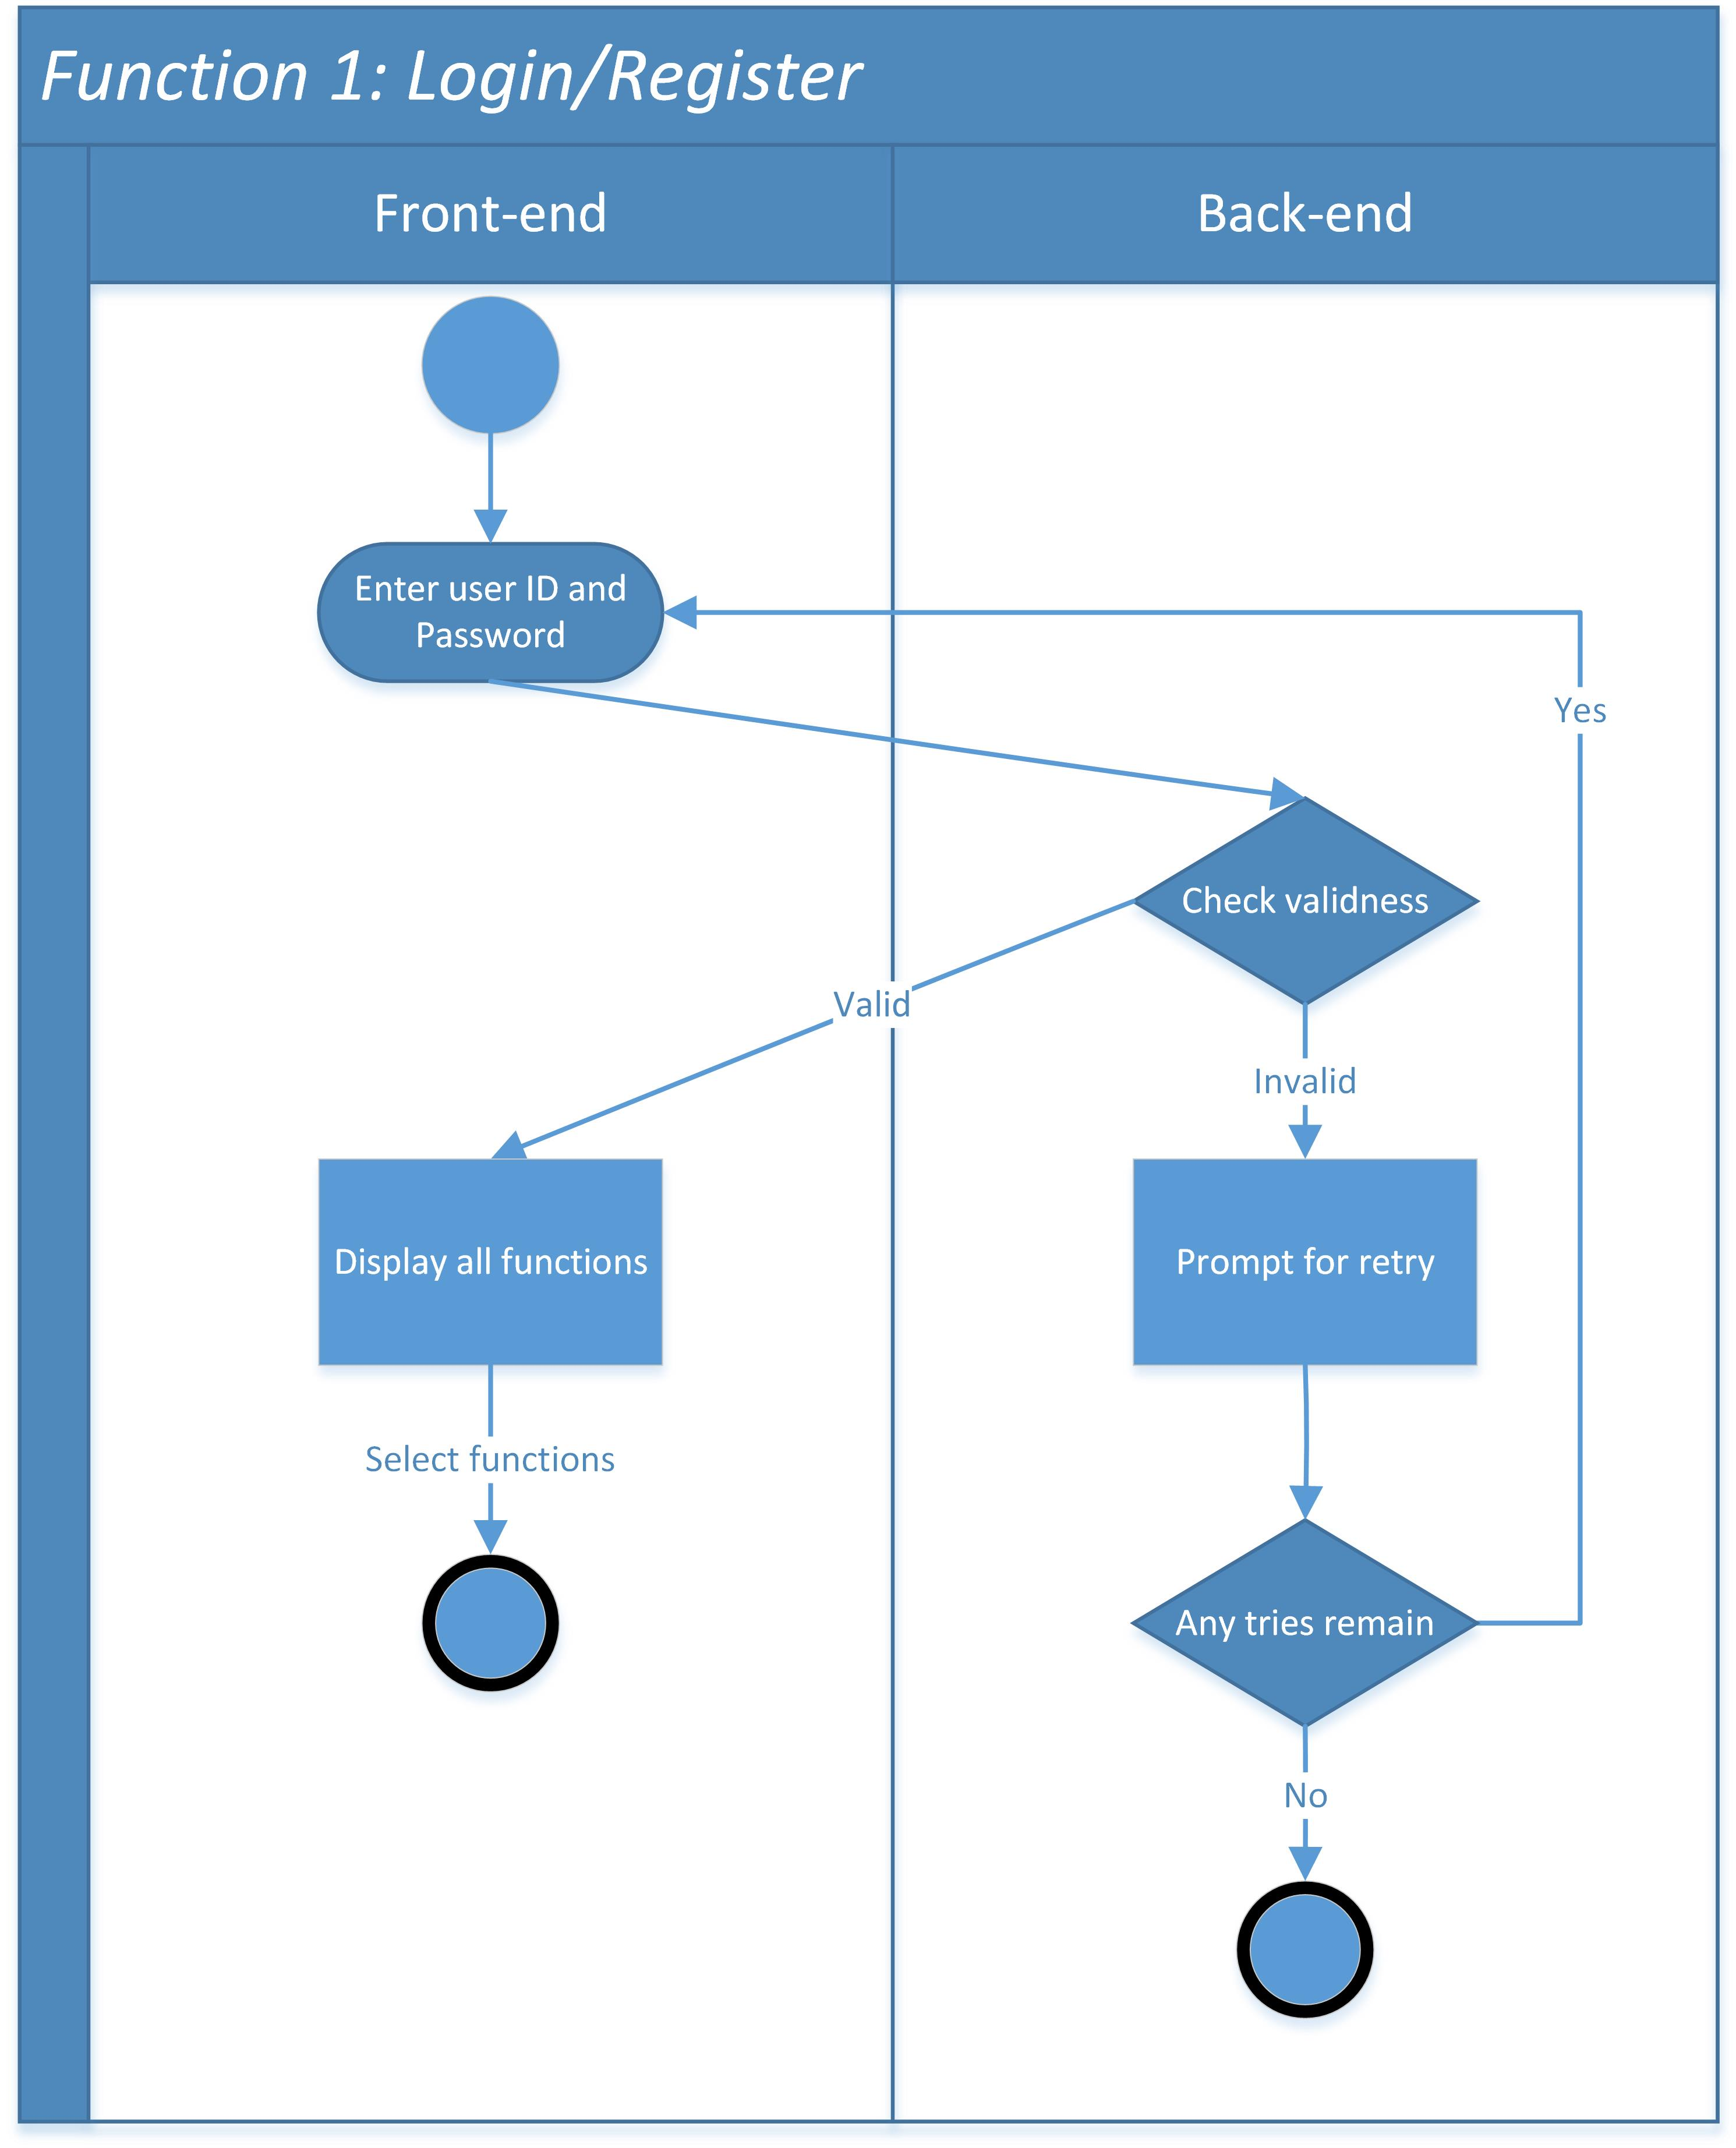
\includegraphics[width=1\columnwidth]{SwimLaneDiagram/Usecase_1.jpg}
\end{figure}
\newpage

\subsection{Diagram 2: Modify Profile}

\begin{figure}[H]
    \centering
    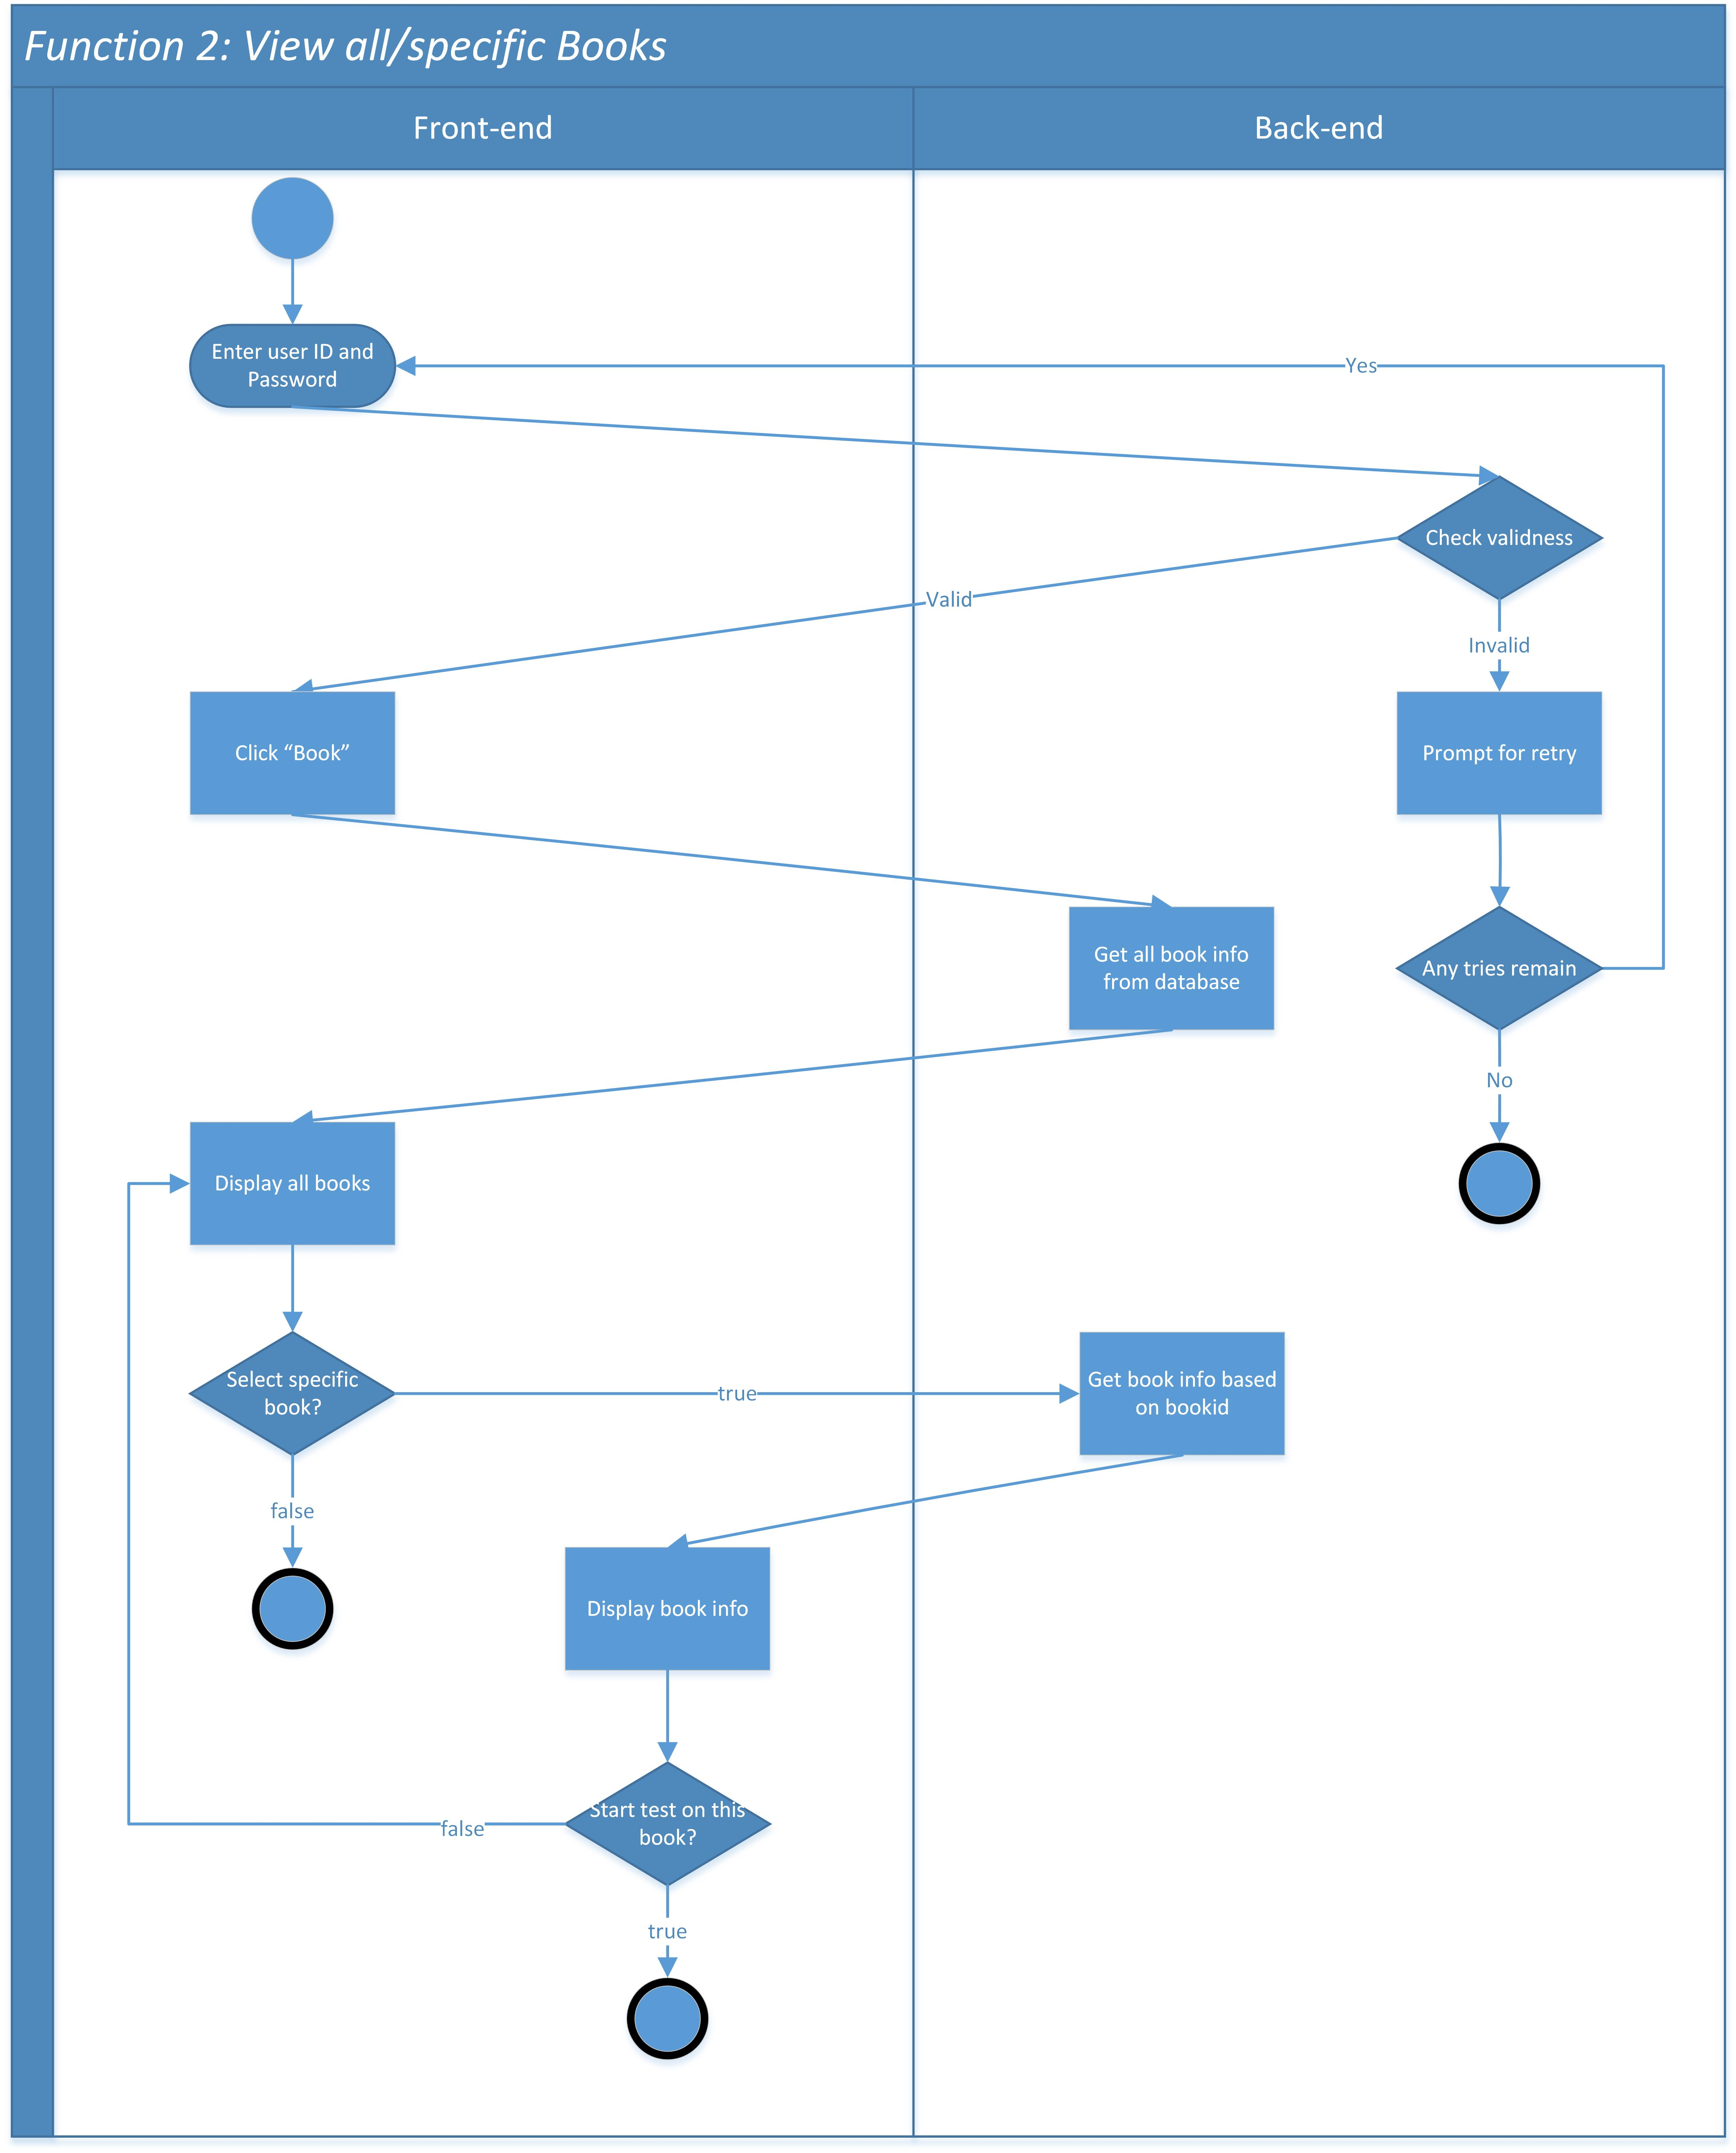
\includegraphics[width=0.8\columnwidth]{SwimLaneDiagram/Usecase_2.jpg}
\end{figure}
\newpage

\subsection{Diagram 3: Access Camera Surveillance}

\begin{figure}[H]
    \centering
    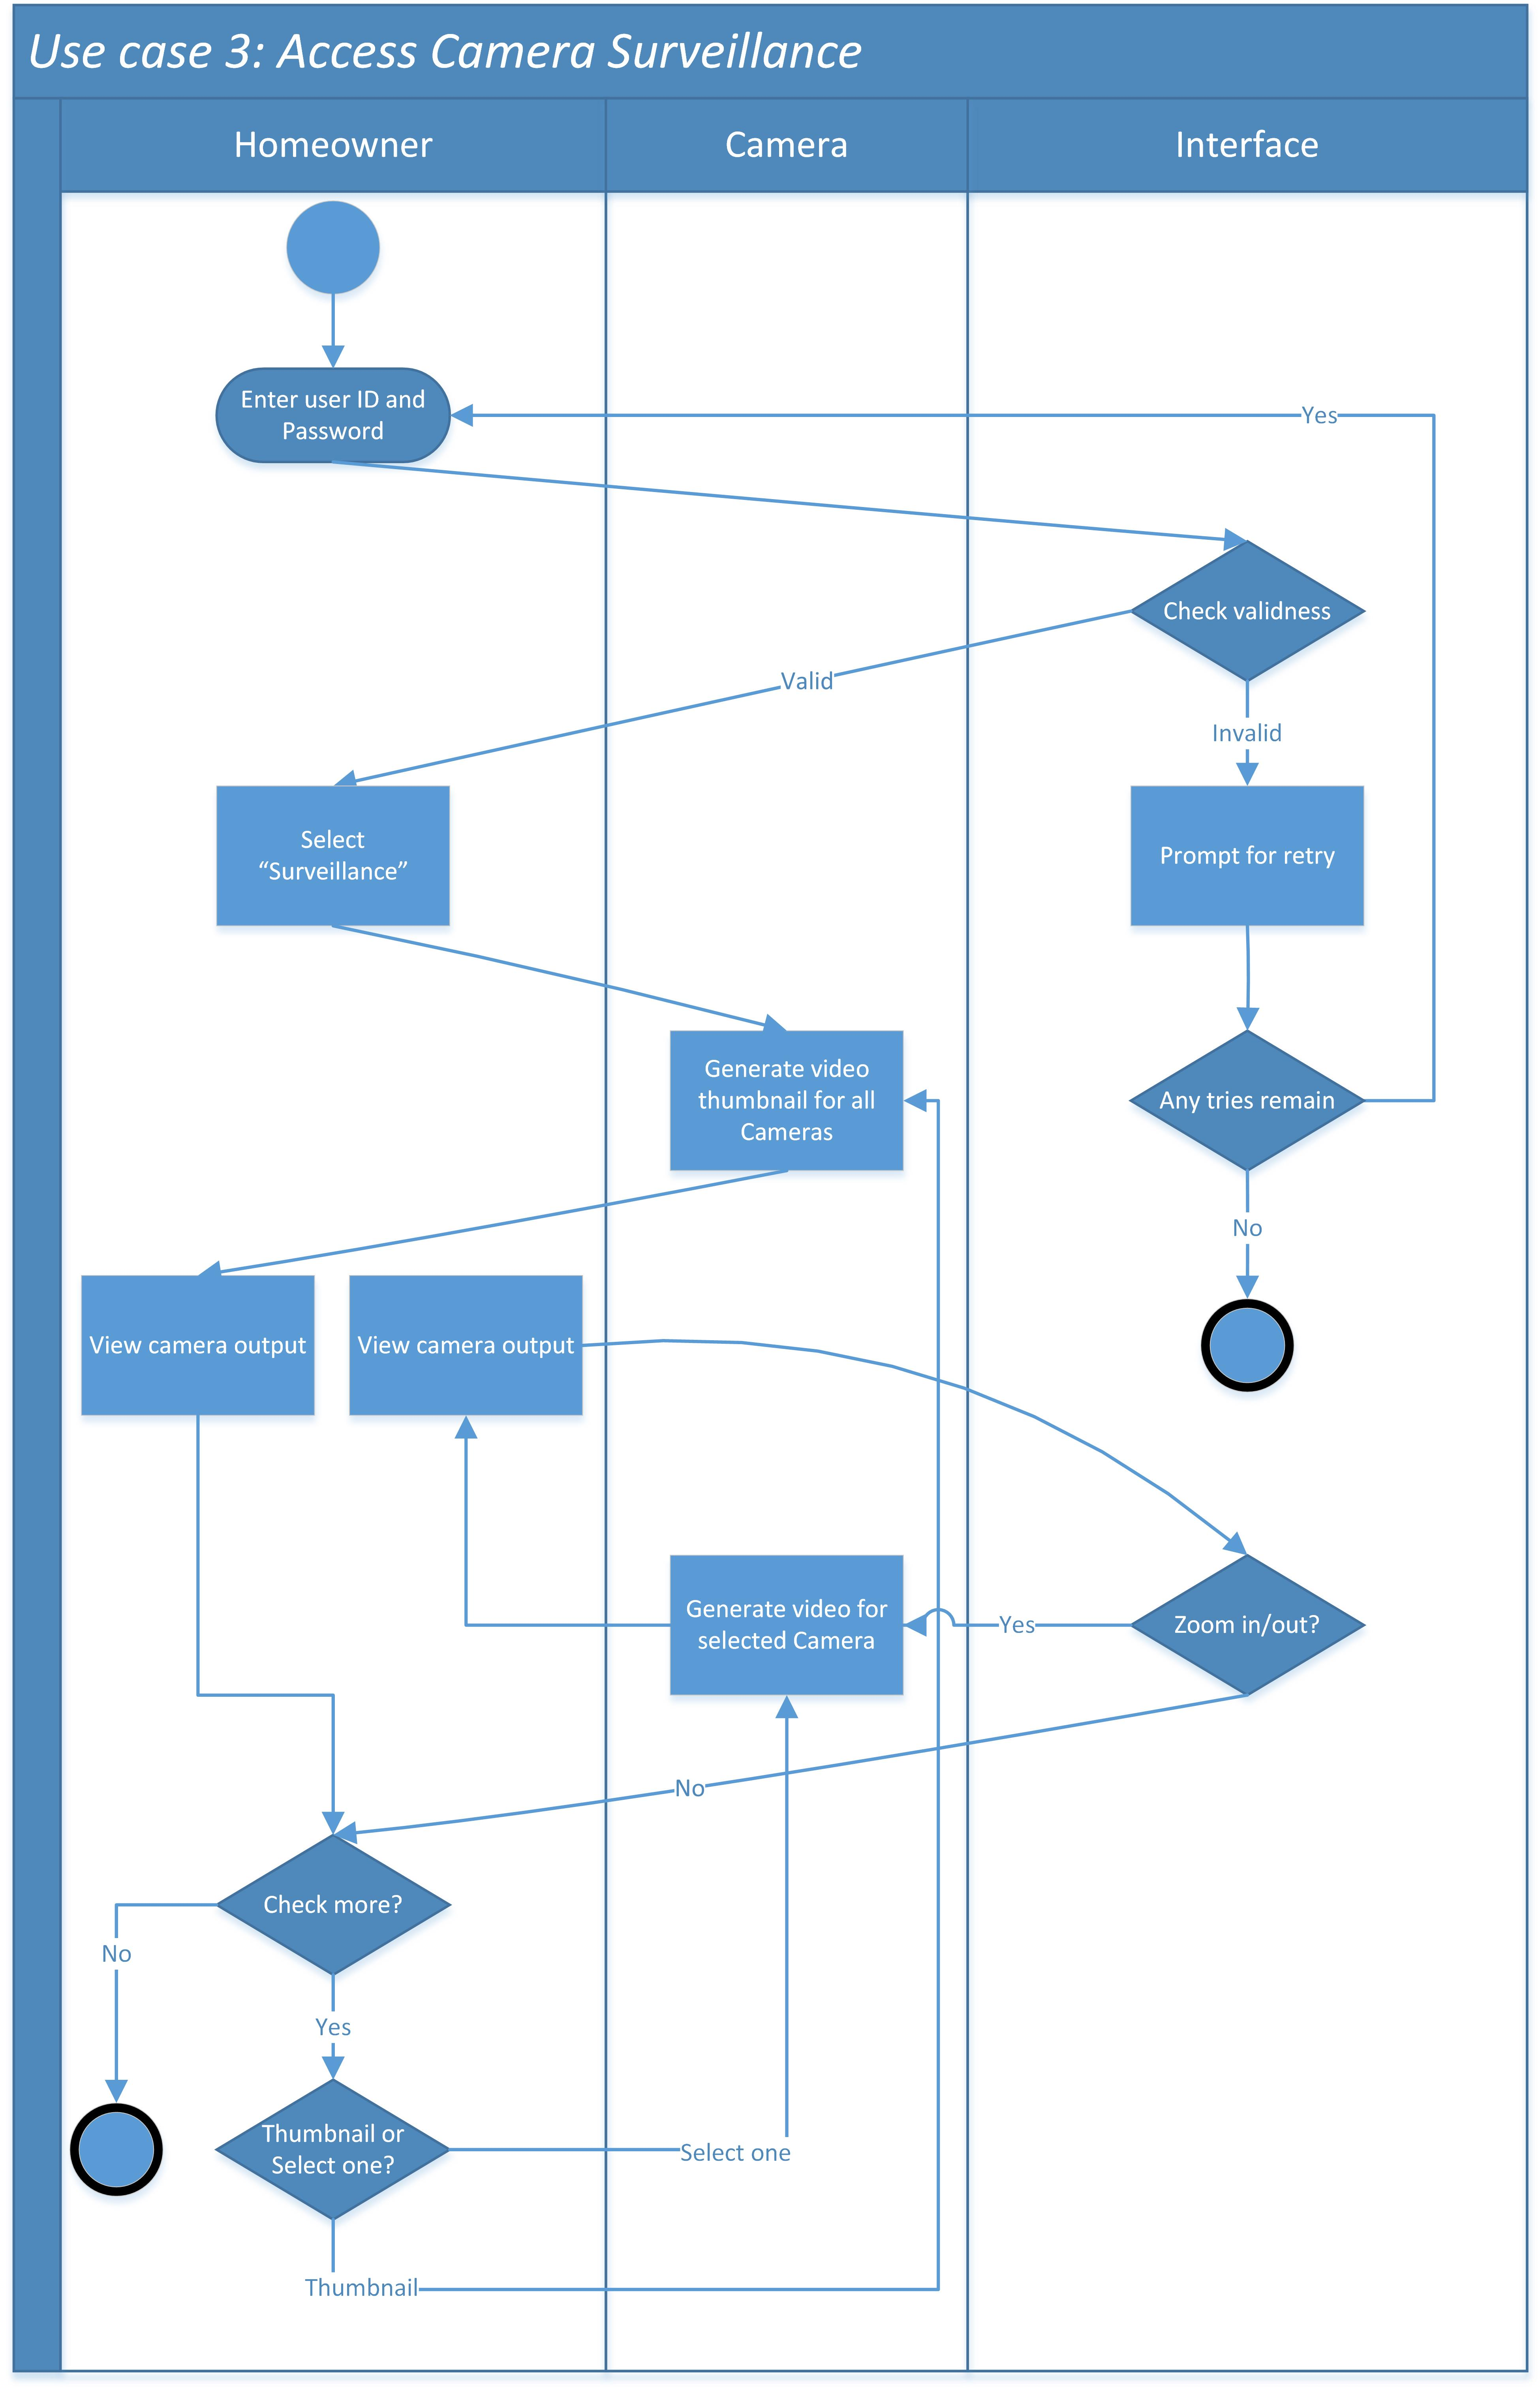
\includegraphics[width=0.85\columnwidth]{SwimLaneDiagram/Usecase_3.jpg}
\end{figure}
\newpage

\subsection{Diagram 4: Activate / Deactivate the Cameras and Sensors}

\begin{figure}[H]
    \centering
    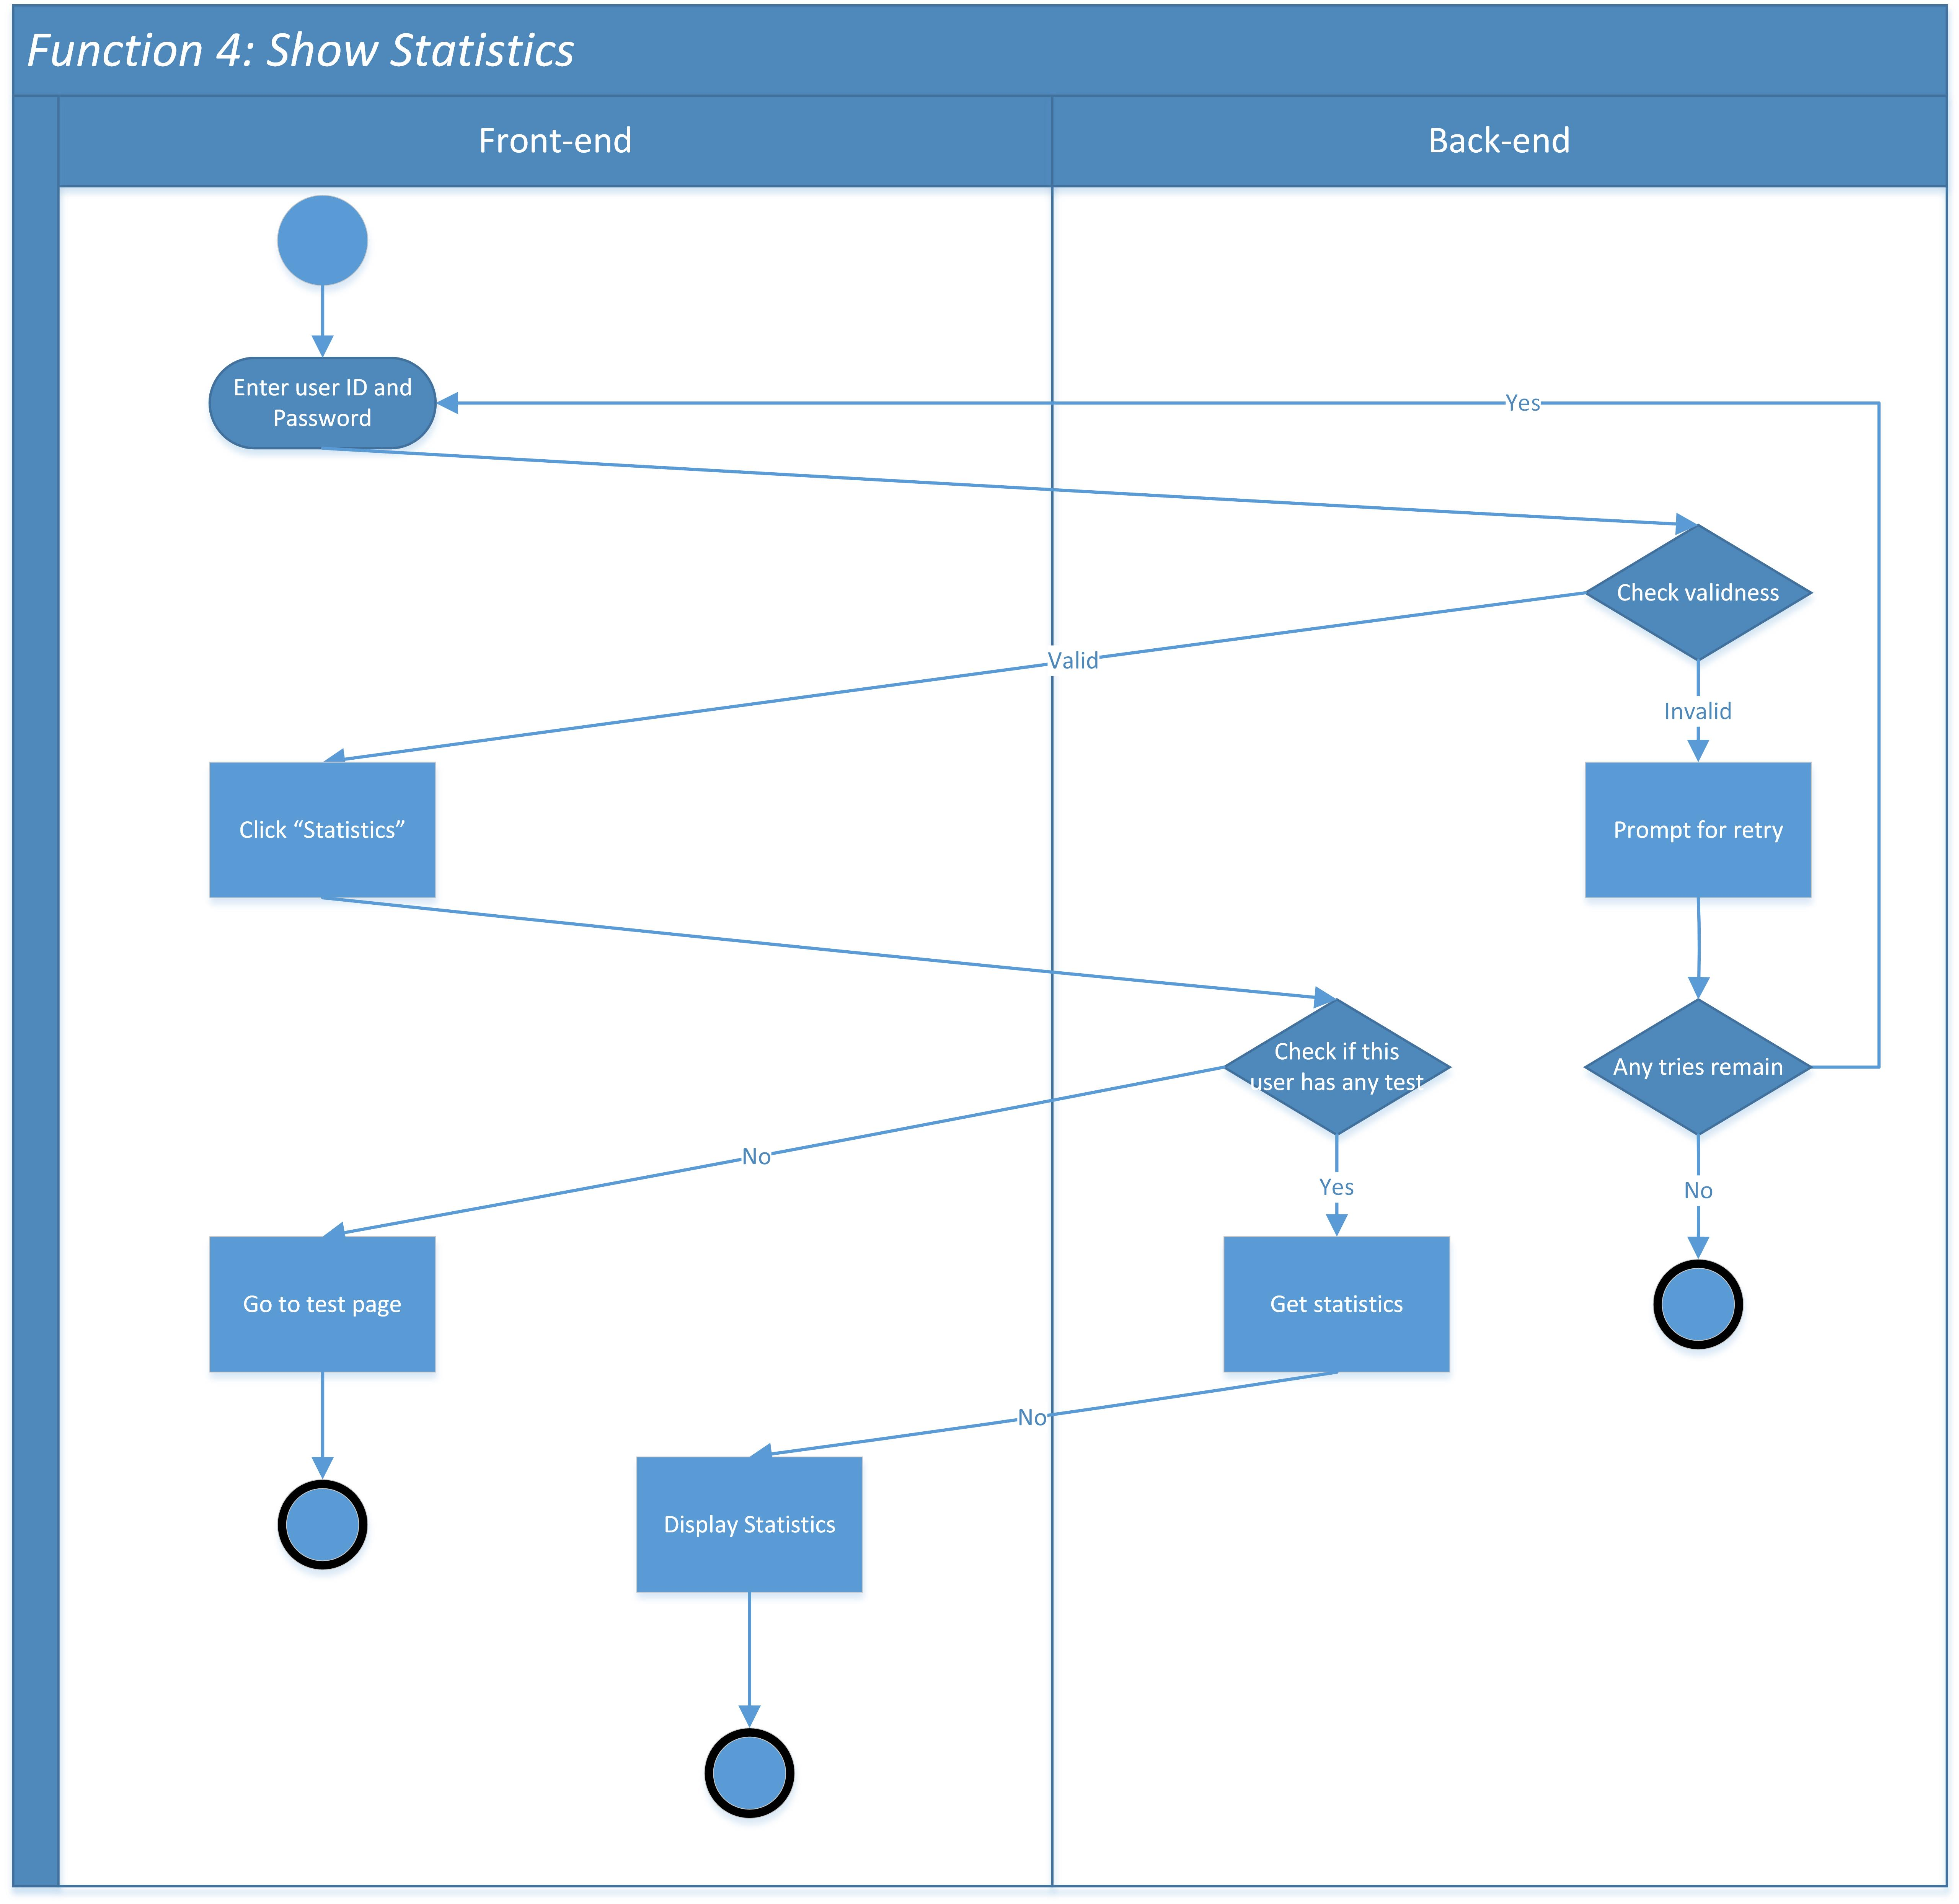
\includegraphics[width=1\columnwidth]{SwimLaneDiagram/Usecase_4.jpg}
\end{figure}
\newpage

\subsection{Diagram 5: Register new Homeowner/Delete Homeowner}
\begin{figure}[H]
    \centering
    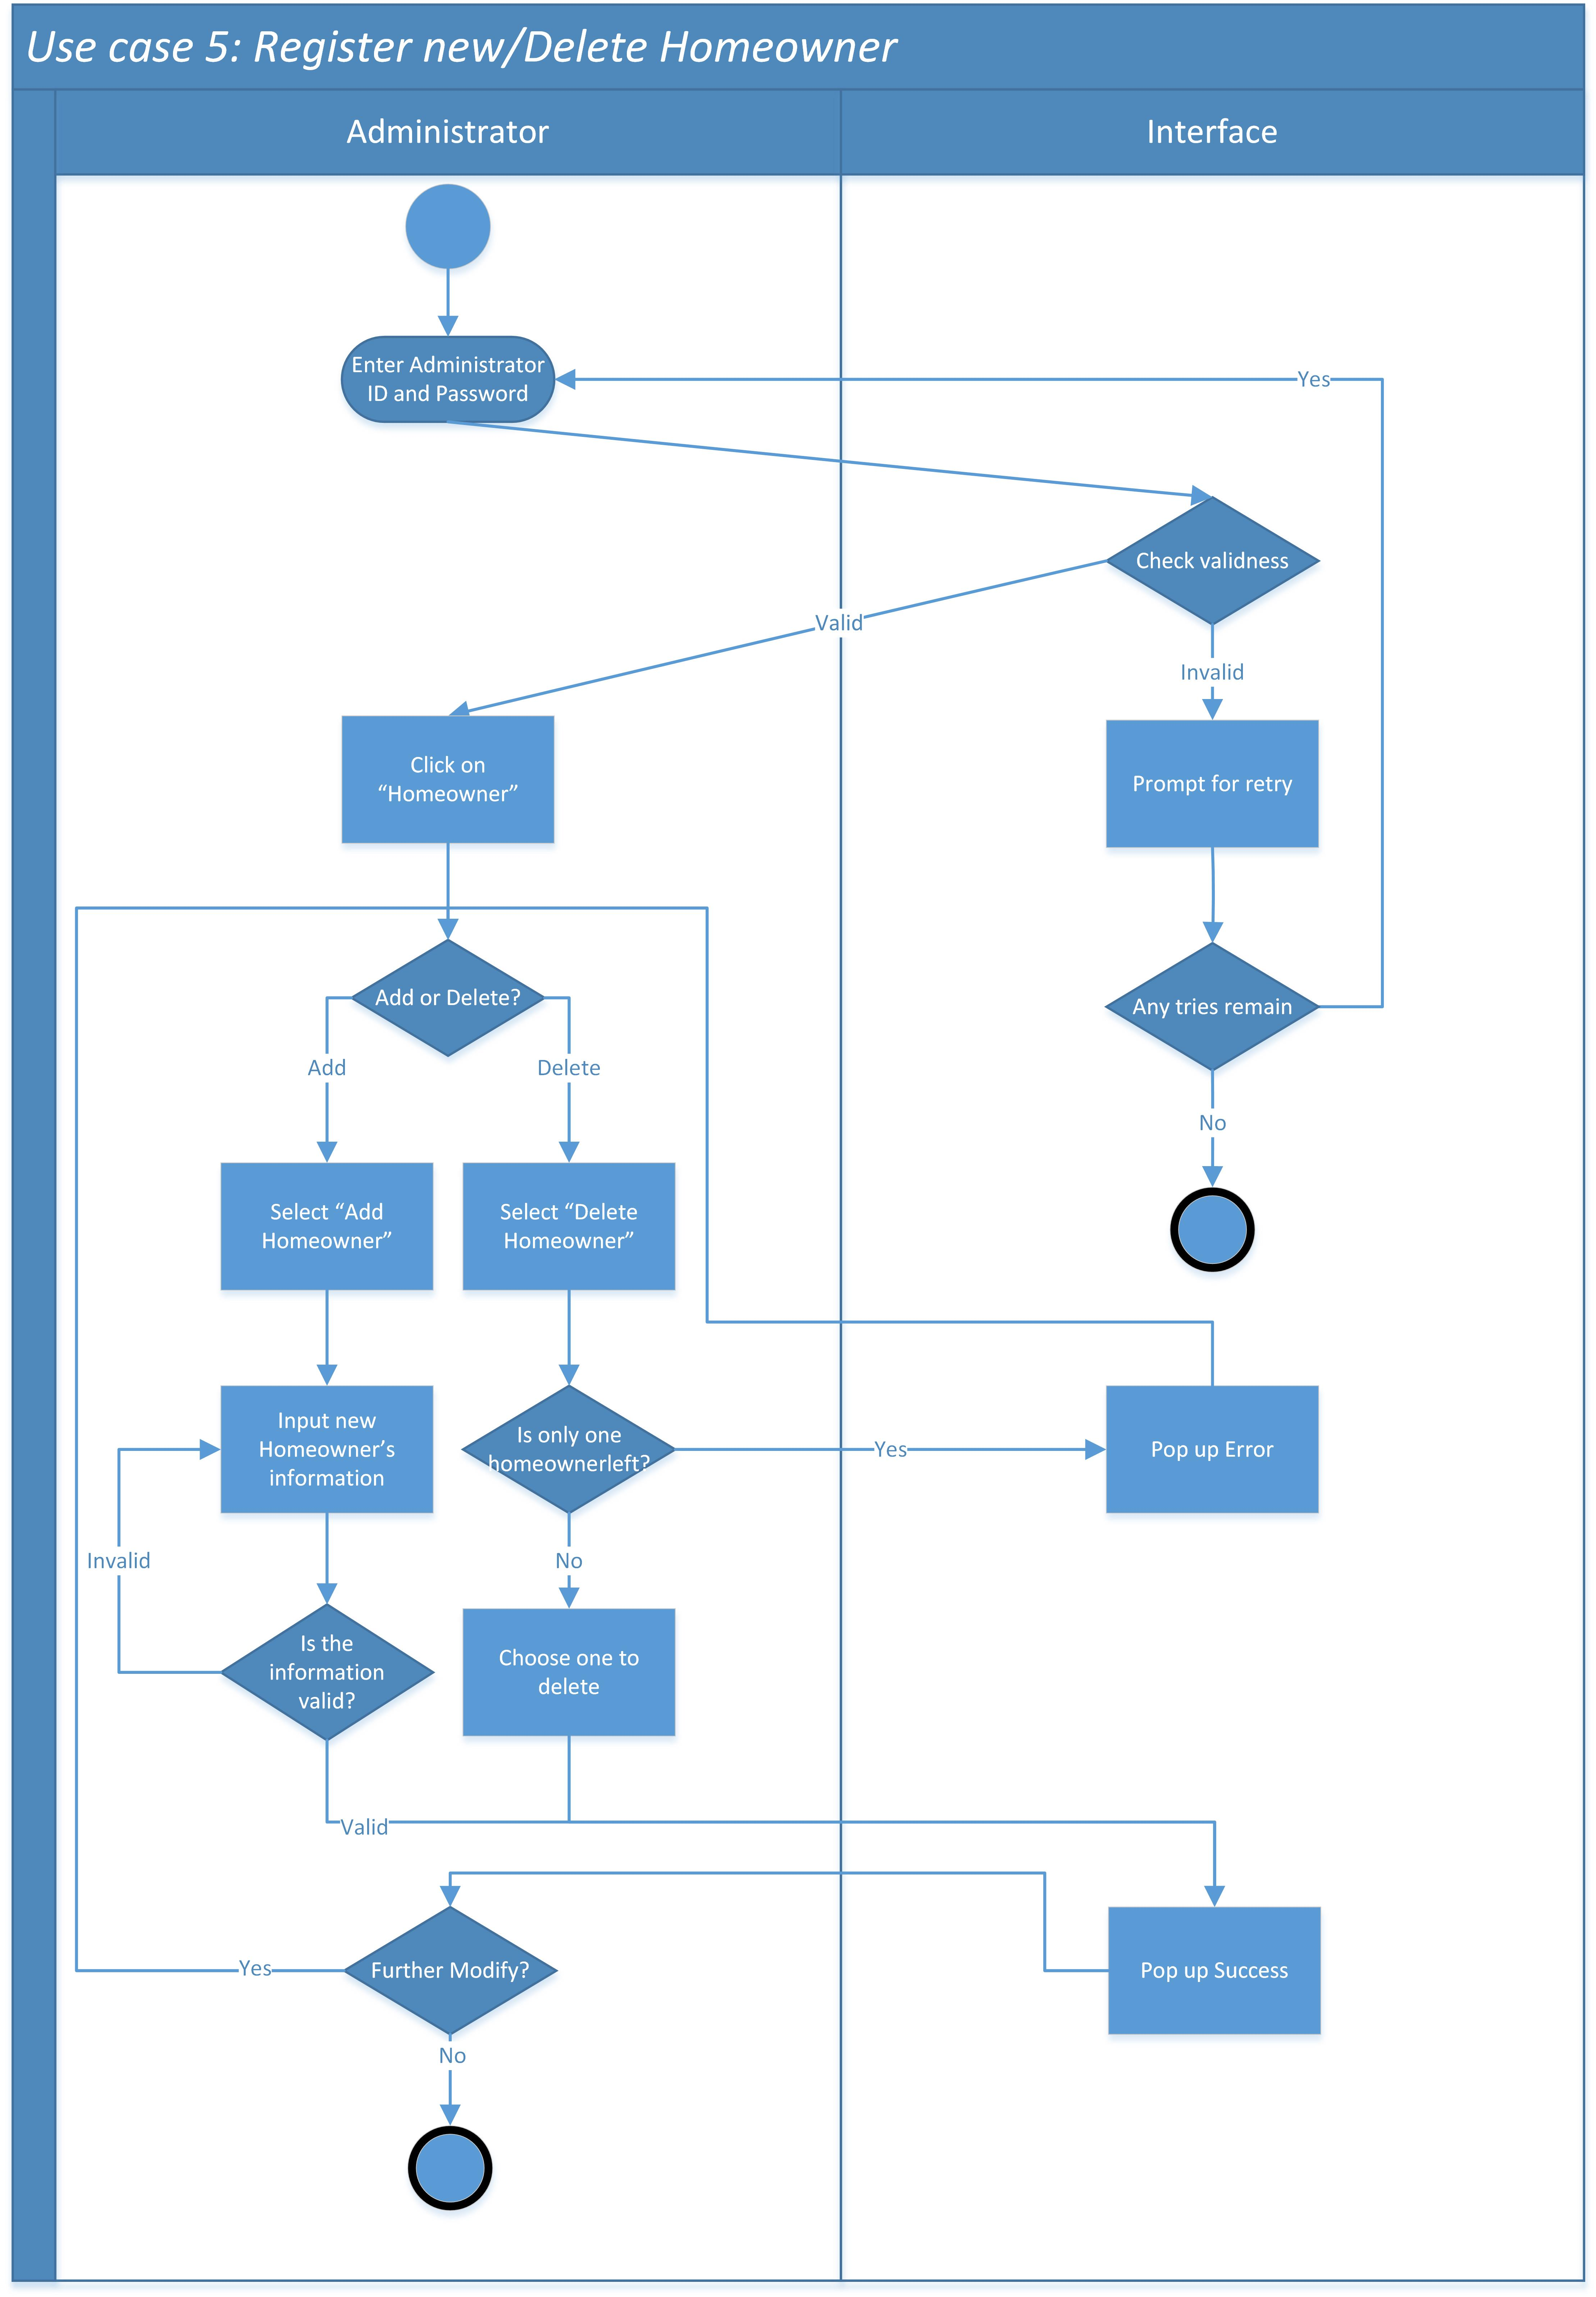
\includegraphics[width=0.9\columnwidth]{SwimLaneDiagram/Usecase_5.jpg}
\end{figure}
\newpage

\subsection{Diagram 6: Add/Remove Camera or Sensor}
\begin{figure}[H]
    \centering
    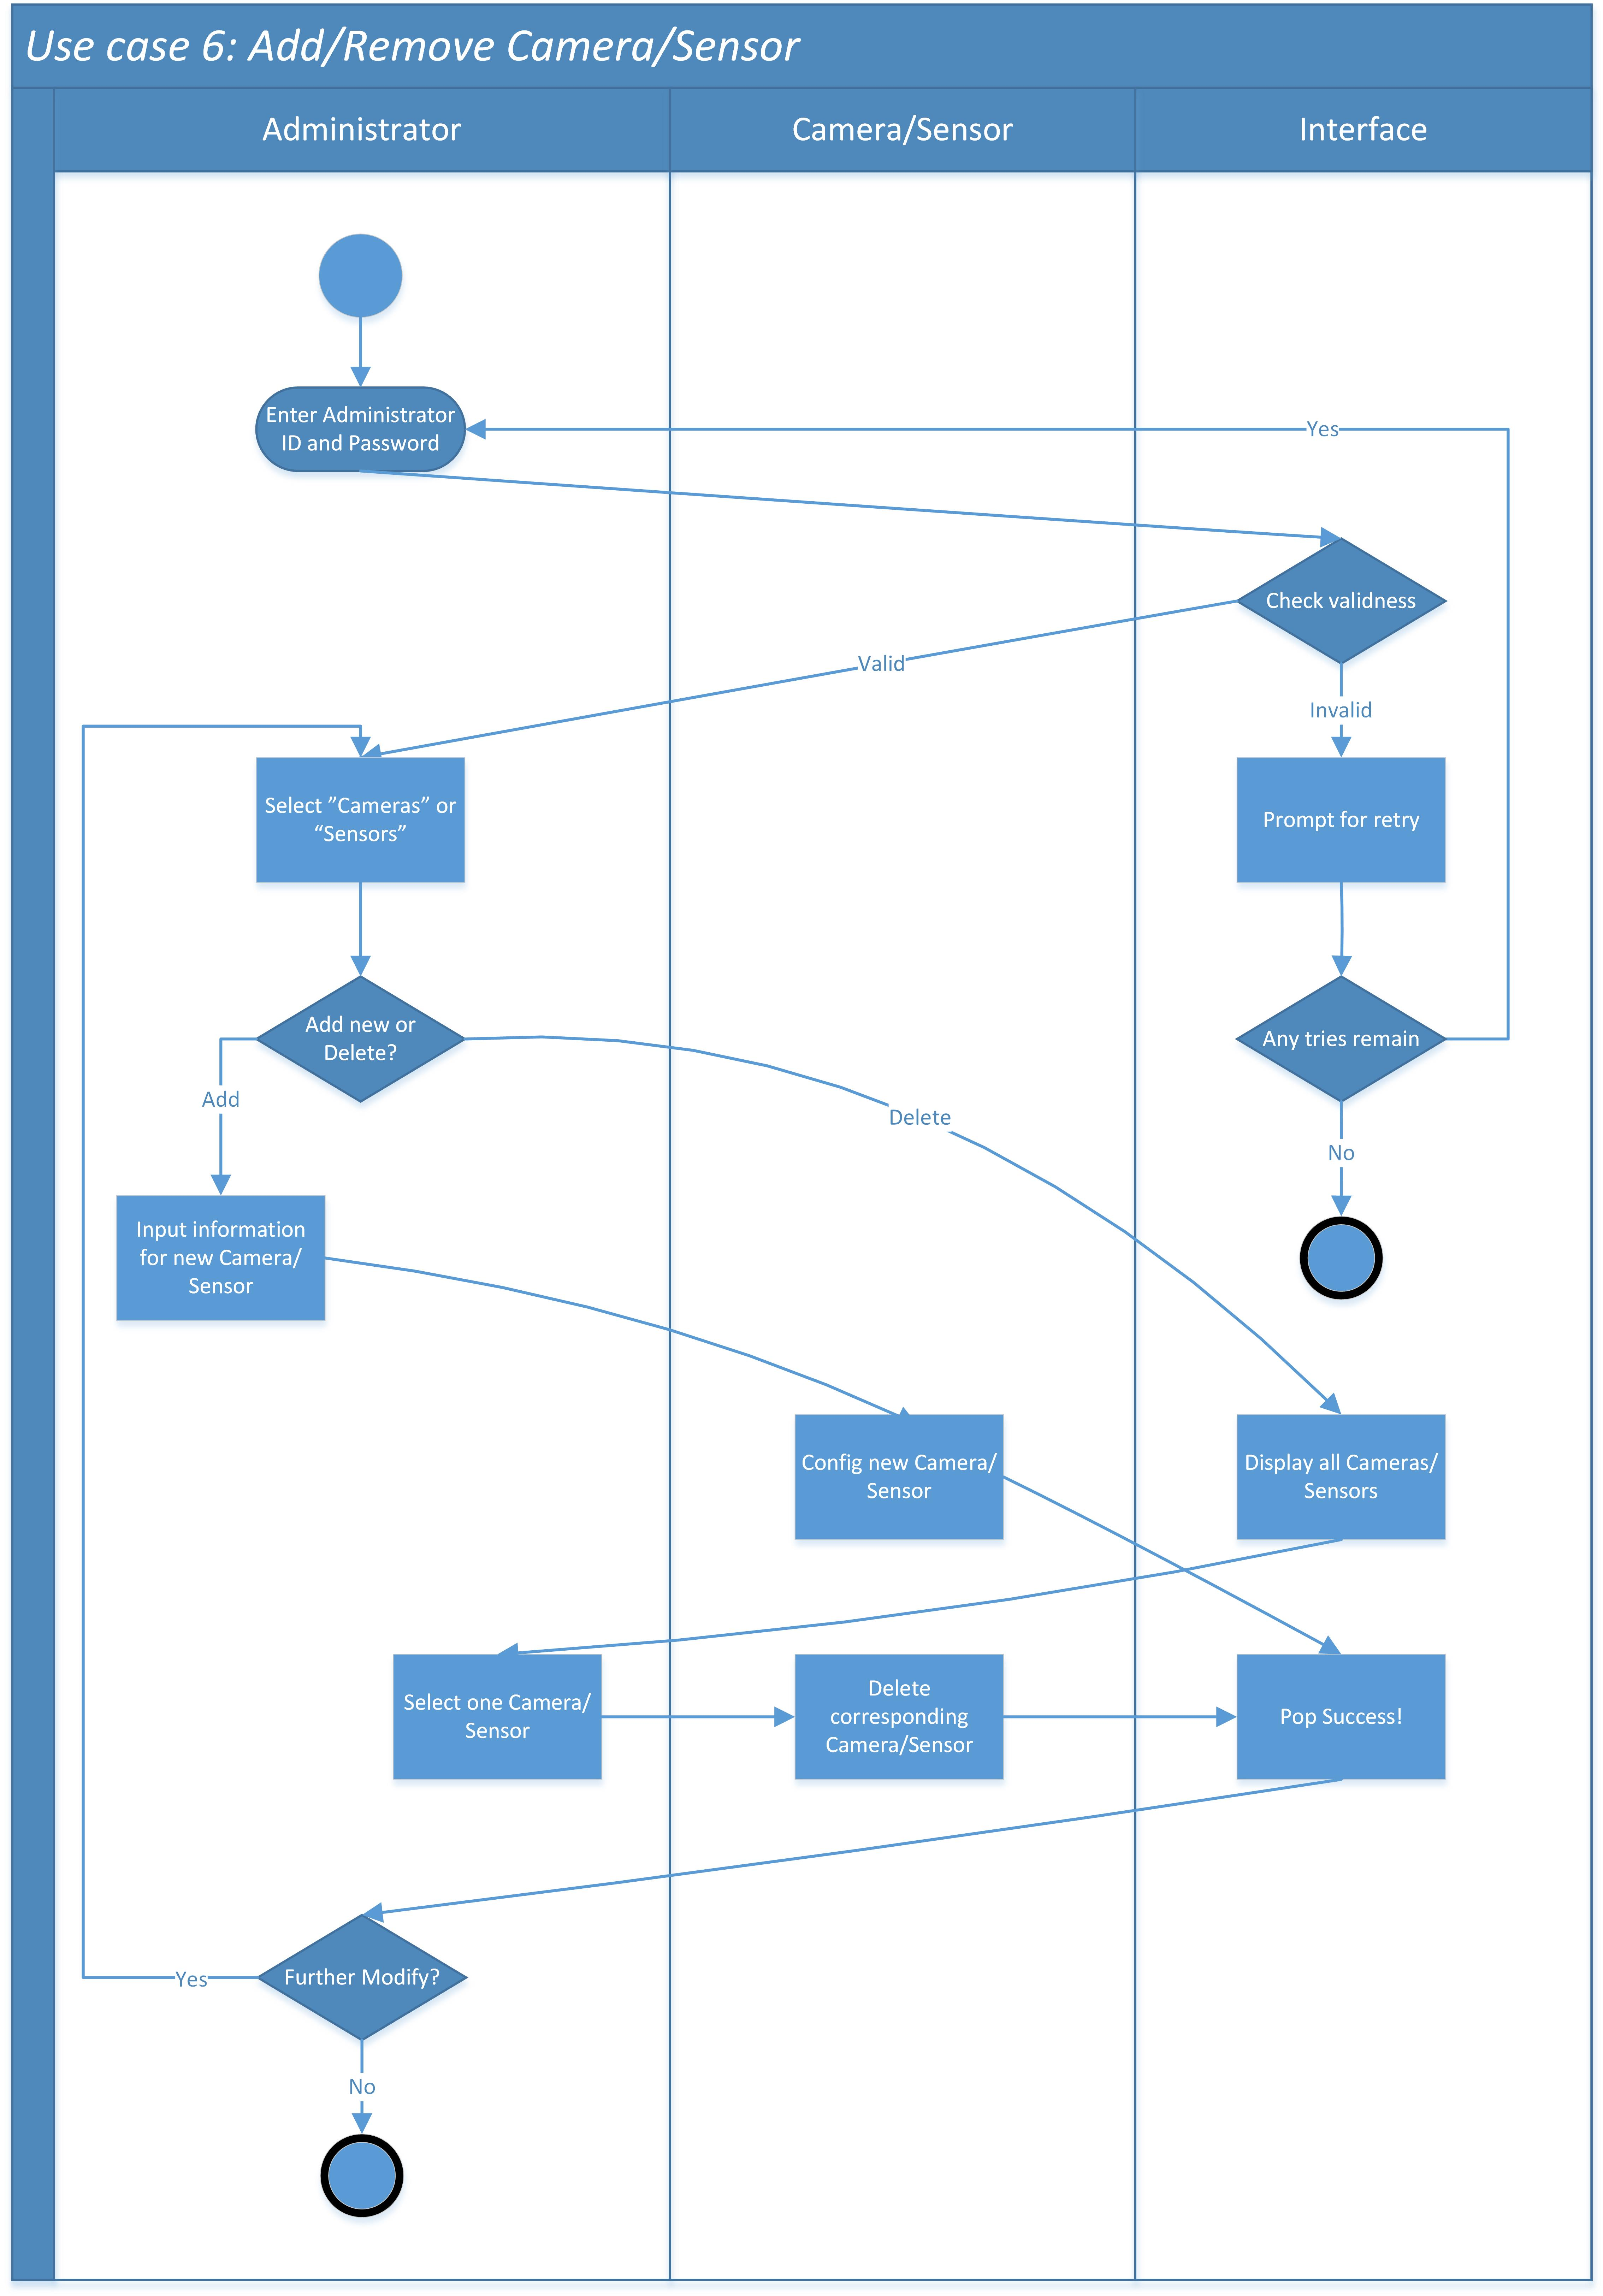
\includegraphics[width=0.9\columnwidth]{SwimLaneDiagram/Usecase_6.jpg}
\end{figure}
\newpage

\subsection{Diagram 7: Contact Homeowneror Emergency service when Emergency occurs}
\begin{figure}[H]
    \centering
    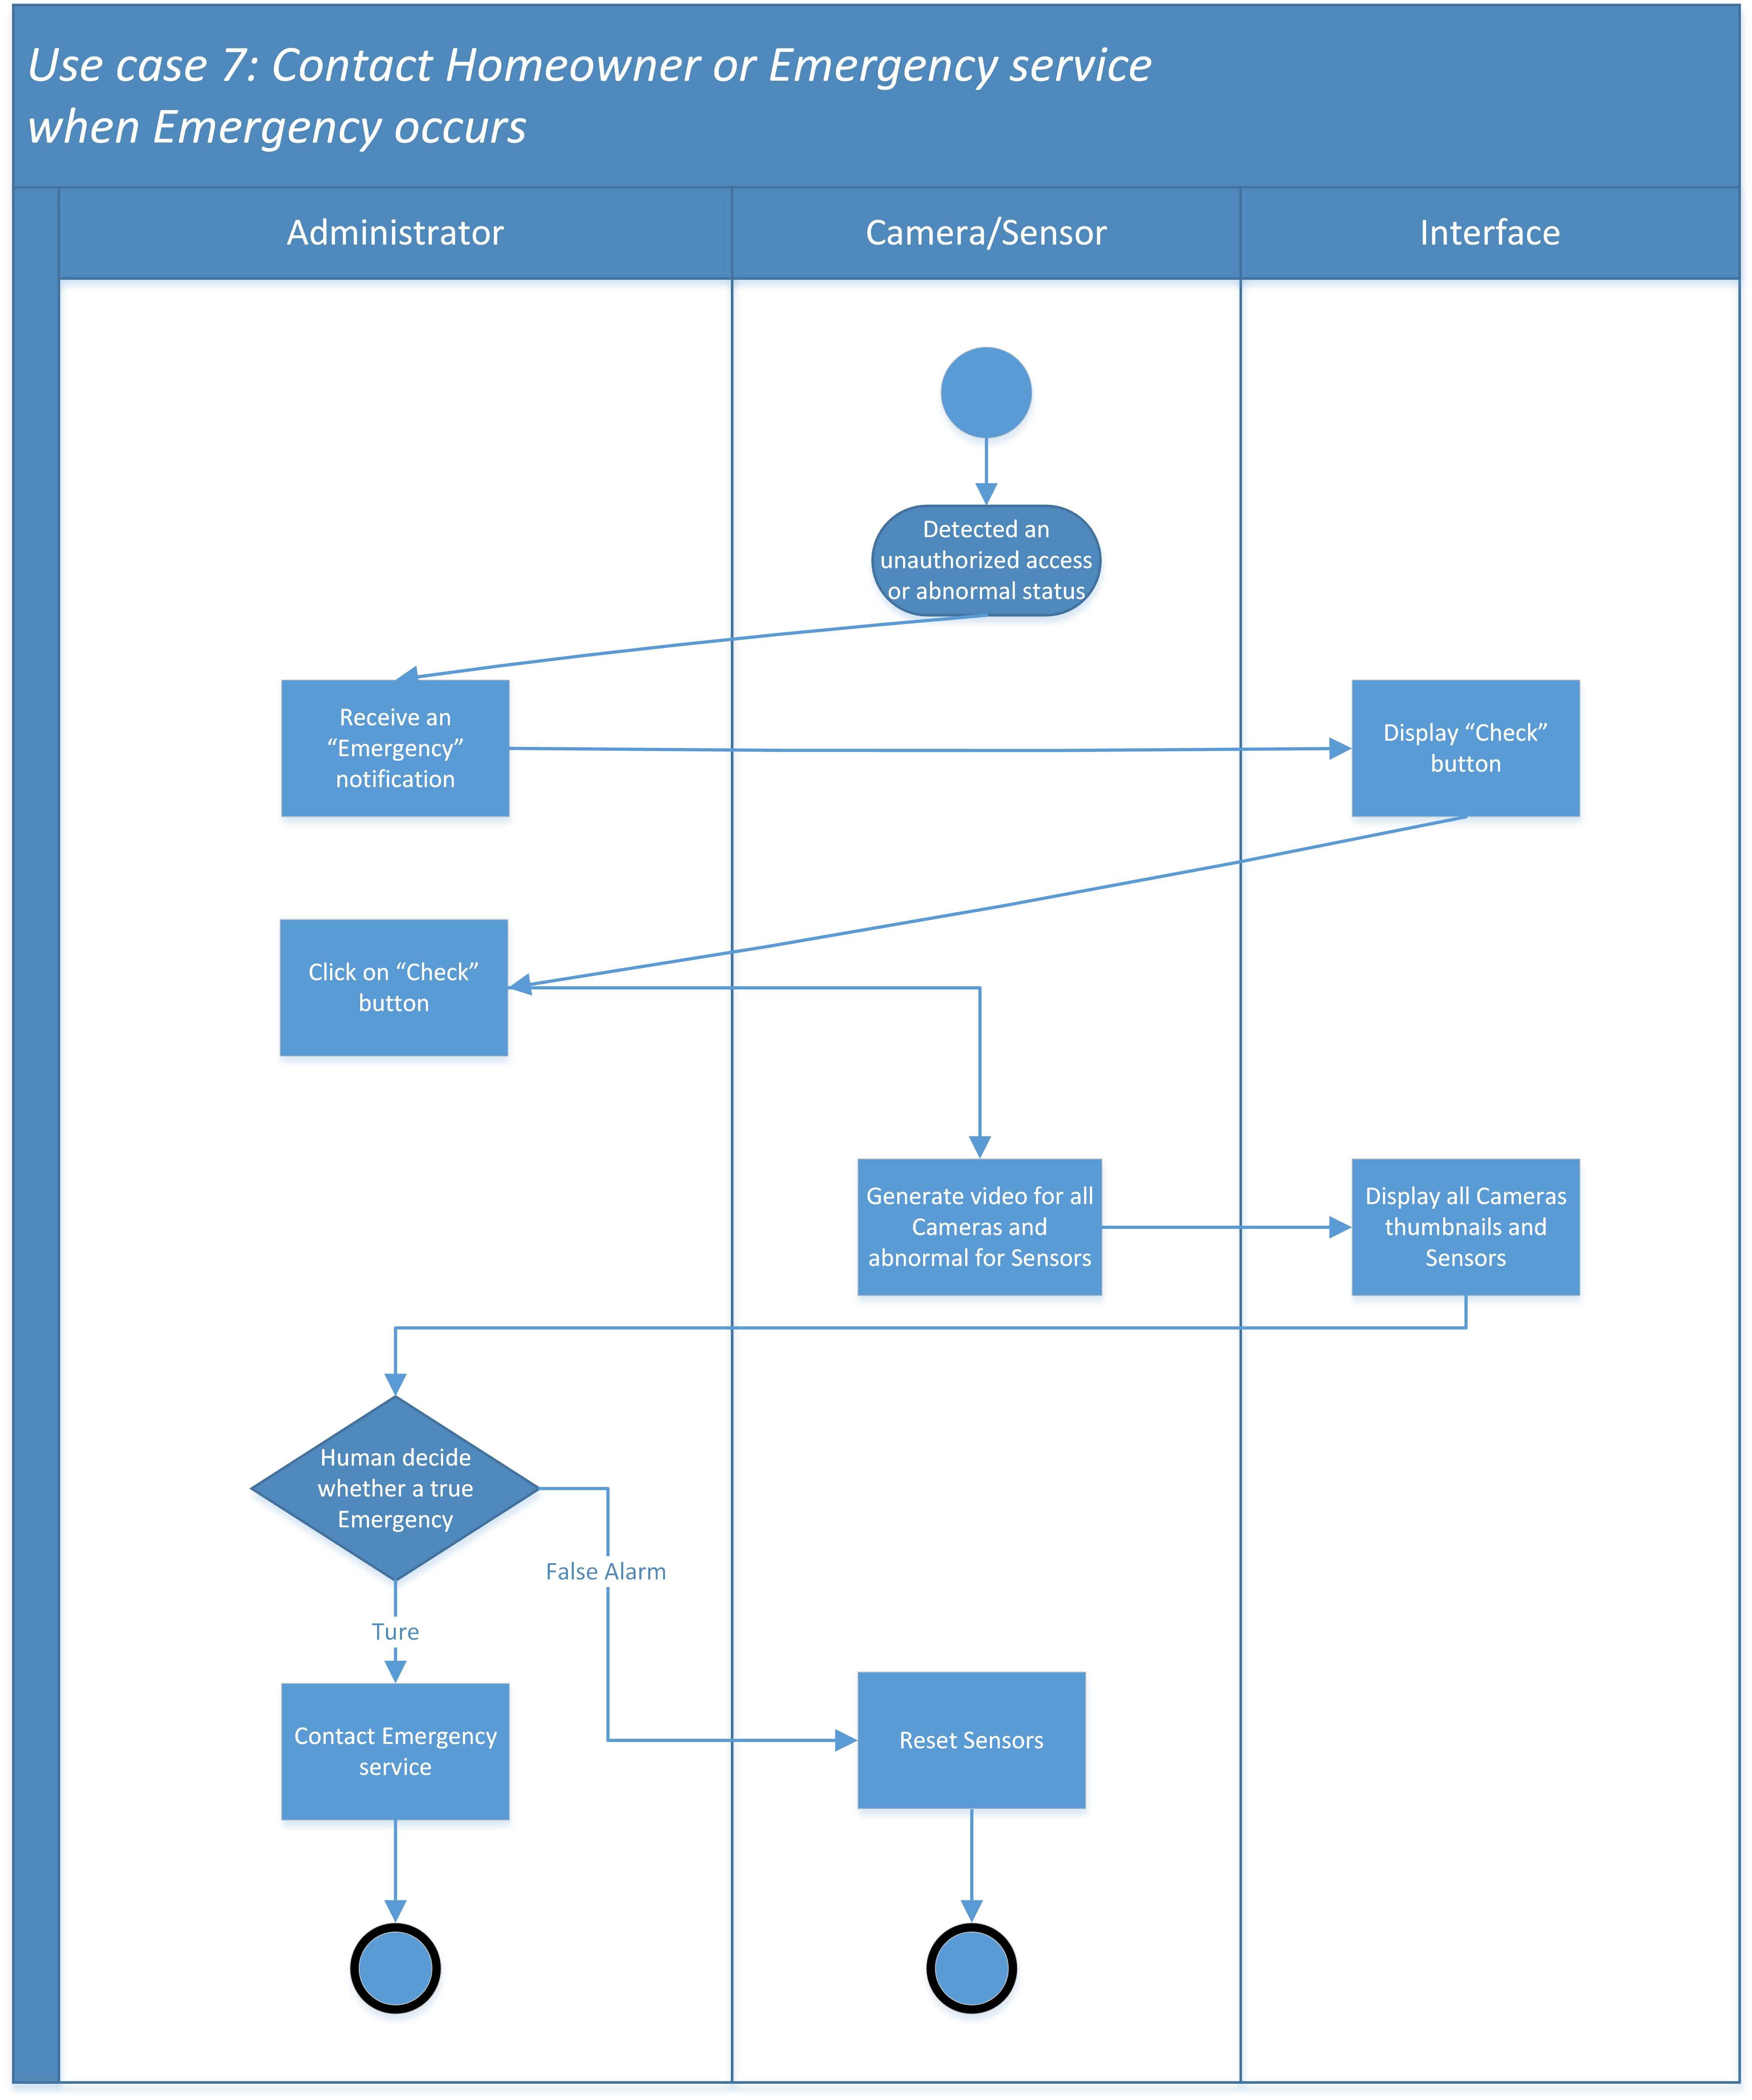
\includegraphics[width=0.8\columnwidth]{SwimLaneDiagram/Usecase_7.jpg}
\end{figure}
\vskip 0.2in

\phantomsection\addcontentsline{toc}{section}{Reference}\tolerance=500
\bibliography{references/references}

\end{document}
